%%%%%%%%%%%%%%%%%%%%%%%%%%%%%%%%%%%%%%%%%
% Beamer Presentation
% LaTeX Template
% Version 1.0 (10/11/12)
%
% This template has been downloaded from:
% http://www.LaTeXTemplates.com
%
% License:
% CC BY-NC-SA 3.0 (http://creativecommons.org/licenses/by-nc-sa/3.0/)
%
%%%%%%%%%%%%%%%%%%%%%%%%%%%%%%%%%%%%%%%%%

%----------------------------------------------------------------------------------------
%	PACKAGES AND THEMES
%----------------------------------------------------------------------------------------

\documentclass{beamer}

\mode<presentation> {
	\usetheme{Madrid}
}

\usepackage{graphicx} % Allows including images
\usepackage{booktabs} % Allows the use of \toprule, \midrule and \bottomrule in tables

\usepackage{listings}
\usepackage{xcolor}

\definecolor{codegreen}{rgb}{0,0.6,0}
\definecolor{codegray}{rgb}{0.5,0.5,0.5}
\definecolor{codepurple}{rgb}{0.58,0,0.82}
\definecolor{backcolour}{rgb}{0.95,0.95,0.92}

\lstdefinestyle{mystyle}{
	backgroundcolor=\color{backcolour},   
	commentstyle=\color{codegreen},
	keywordstyle=\color{magenta},
	numberstyle=\tiny\color{codegray},
	stringstyle=\color{codepurple},
	basicstyle=\ttfamily\footnotesize,
	breakatwhitespace=false,         
	breaklines=true,                 
	captionpos=b,                    
	keepspaces=true,                 
	numbers=left,                    
	numbersep=5pt,                  
	showspaces=false,                
	showstringspaces=false,
	showtabs=false,                  
	tabsize=2,
	basicstyle=\tiny
}

\lstset{style=mystyle}


%----------------------------------------------------------------------------------------
%	TITLE PAGE
%----------------------------------------------------------------------------------------

\title[Microservices in Action]{Microservices Architecture "The new normal"} % The short title appears at the bottom of every slide, the full title is only on the title page

\author{Mohamed Sweelam} % Your name
\institute[etisalat UAE] % Your institution as it will appear on the bottom of every slide, may be shorthand to save space
{
	Senior Software Engineer \\
	\medskip
	\textit{mohamedsweelam@fci.helwan.edu.eg} % Your email address
}
\date{\today} % Date, can be changed to a custom date


\usefonttheme{professionalfonts}
\begin{document}
	
	\begin{frame}
	\titlepage
\end{frame}

\begin{frame}
	\frametitle{Objectives} % Table of contents slide, comment this block out to remove it
		\begin{enumerate}
			\item<1-> \large {Provide good Arabic content for the topic}
			\item<2-> \large {Overview of Microservices}
			\item<3-> \large {Move step forwards towards recent cloud tools}
			\item<4-> \large {Leave your fear, and let's do it}
		\end{enumerate}
\end{frame}

\begin{frame}
\frametitle{Contents} % Table of contents slide, comment this block out to remove it
	\tableofcontents
\end{frame}

%----------------------------------------------------------------------------------------
%	PRESENTATION SLIDES
%----------------------------------------------------------------------------------------

%------------------------------------------------
\section{From Monolithic to Microservices}
	\subsection	{Definition} 
		\begin{frame}
			\frametitle{Definition}
				\begin{block}{Monolithic}
					A monolithic application is self-contained, and independent from other computing applications. The design philosophy is that the application is responsible not just for a particular task, but can perform every step needed to complete a particular function.
				\end{block}
			
			\vspace{5mm}
			\begin{block}{Microservices}
				Microservices is a software development technique that arranges an application as a collection of loosely coupled services. 
			\end{block}
			
			\vspace{10mm}
			\tiny{https://en.wikipedia.org/wiki/Monolithic\_application}\\
			\tiny{https://en.wikipedia.org/wiki/Microservices}		
		\end{frame}
	
	\subsection	{Why Microservices?}
		\begin{frame}
			\frametitle{Why Microservices?}
				\begin{enumerate}
					\item<1-> Unit design
						\begin{itemize}
							\item \scriptsize {The application consists of loosely coupled services}. 
							\item \scriptsize {Each service supports a single business task}.
						\end{itemize}
					\item<2-> Flexibility
						\begin{itemize}
							\item \scriptsize {Each microservice can be developed using a programming language and framework that best suits}.
						\end{itemize}
					\item<3-> Maintainability
						\begin{itemize}
							\item \scriptsize {Simple, focused, and independent. So the application is easier to maintain}.
						\end{itemize}
					\item<4-> Resiliency
						\begin{itemize}
							\item \scriptsize {The application functionality is distributed across multiple services}. 
							\item \scriptsize {If a microservice fails, the functionality offered by the others continues to be available}.
						\end{itemize}
					\item<5-> Scalability
						\begin{itemize}
							\item \scriptsize {Each microservice can be scaled independently of the other services}.
						\end{itemize}
				\end{enumerate}
		\end{frame}

	\subsection {Microservices vs Monolithic}
		\begin{frame}
			\frametitle{Microservices vs Monolithic}
				\begin{figure}[h]
					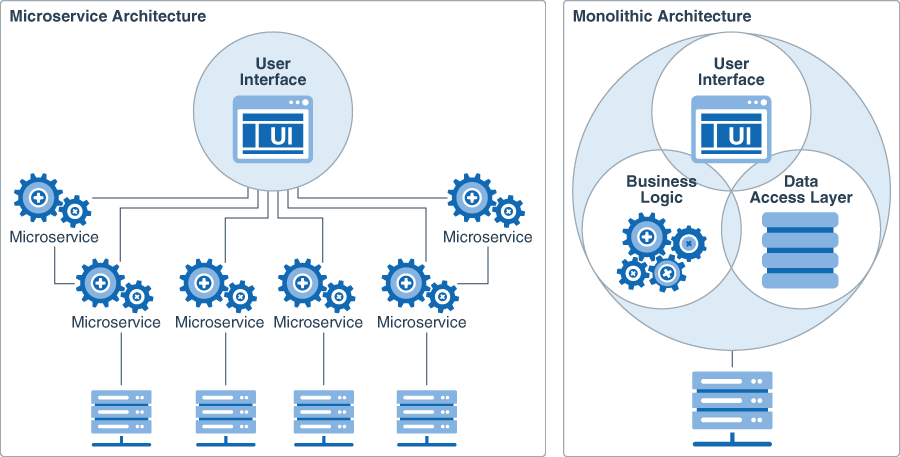
\includegraphics[width=0.8\linewidth]{img/monolithic_vs_microservice.png}
					\caption{mivroservices vs monolithic}
				\end{figure}
				
				
				\tiny{https://docs.oracle.com/en/solutions/learn-architect-microservice/index.html}		
		\end{frame}

		\begin{frame}
			\frametitle{Closer Look}
				\begin{figure}[h]
					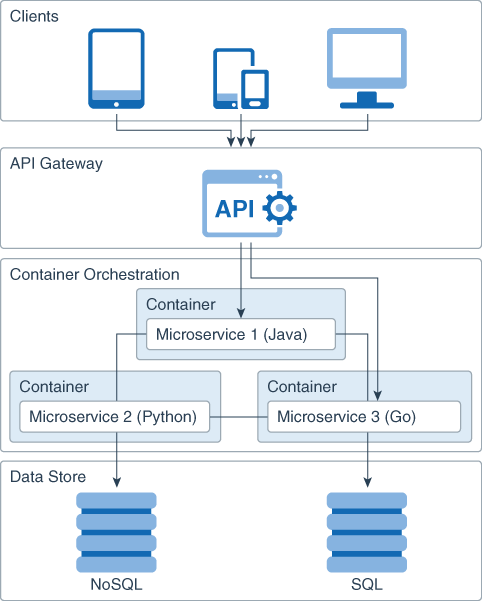
\includegraphics[width=55mm, height=60mm, scale=1]{img/microservice_architecture.png}
					\caption{Microservices In Depth}
				\end{figure}
				
				
				\tiny{https://docs.oracle.com/en/solutions/learn-architect-microservice/index.html}	
		\end{frame}
	
	\subsection {Microservices Architecture}
		\begin{frame}
			\frametitle{Microservices Architecture}
				\begin{figure}[h]
					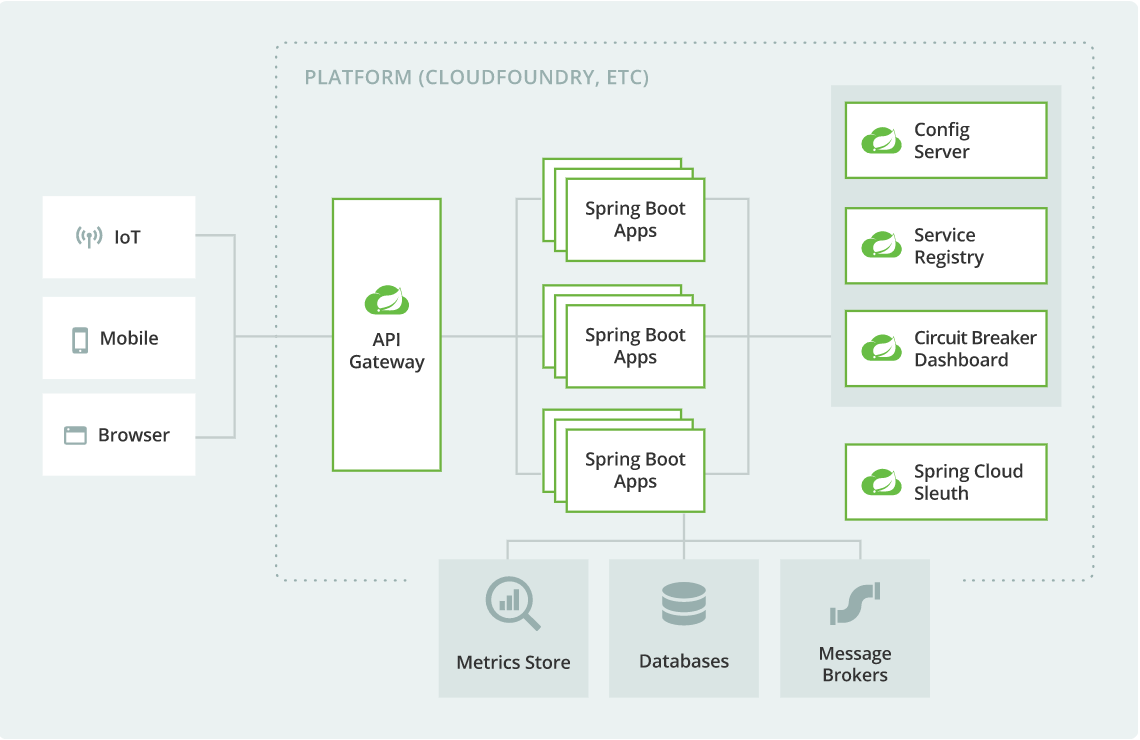
\includegraphics[width=100mm, scale=2]{img/microservice-diagrame.png}
					\caption{Microservices with Spring Cloud}
				\end{figure}\vspace{20mm}

				\tiny{https://spring.io/microservices}	
		\end{frame}
	
		\begin{frame}
			\frametitle{Microservice characteristics}
				\begin{columns}[c]
					\column{.40\textwidth} 
						\hspace{2mm} \textbf {Single Responsibility}
						\begin{itemize}
							\item Business Boundary
							\item Function Boundary
						\end{itemize}
					
					\column{.70\textwidth} % Right column and width
						\begin{figure}[h]
							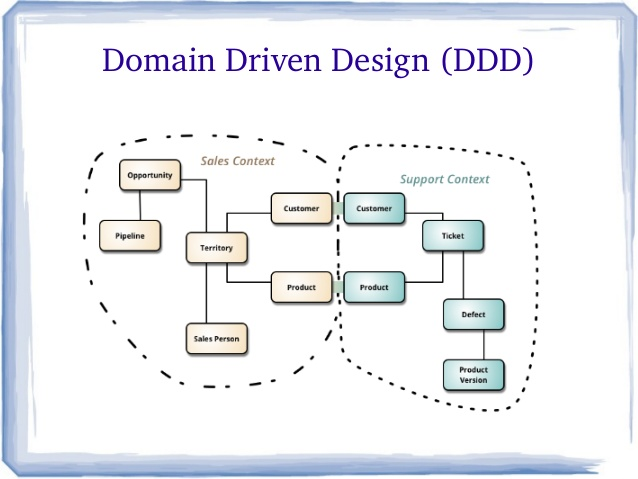
\includegraphics[width=70mm, height=50mm, scale=1]{img/ddd.jpg}
						\end{figure}\vspace{1mm}
				\end{columns}
			
			\vspace{10mm}
			\tiny{https://martinfowler.com/bliki/BoundedContext.html}
		\end{frame}


%--------------------------------------------------
\section {Microservices Core Principles}
	\subsection {Communication Design}
		\begin{frame}
			\frametitle{Communication Design}
				\begin{block} {HTTP communication}
					Also known as \textbf{Synchronous communication}, the calls between services is a viable option for \textbf{service-to-service} via REST API.
				\end{block}
				
				\vspace{2mm}
				\begin{block} {Message communication}
					Also known as \textbf{Asynchronous communication}, the services push messages to a message broker that other services subscribe to.
				\end{block}
			
			\vspace{2mm}
			\begin{block} {Event-driven communication}
				Another type of \textbf{Asynchronous communication}, the services does not need to know the common message structure. Communication between services takes place via events that individual services produce.
			\end{block}
		
		\vspace{5mm}
		\tiny {https://blog.logrocket.com/methods-for-microservice-communication}
		\end{frame}
	
	\begin{frame}
		\frametitle{HTTP communication}
			\begin{figure}[h]
				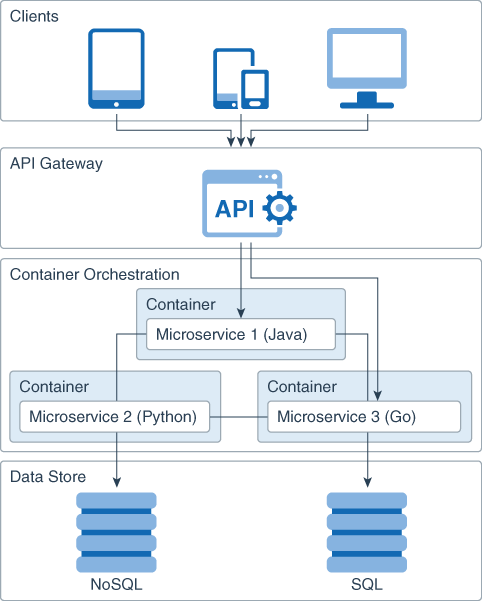
\includegraphics[width=55mm, scale=1]{img/microservice_architecture.png}
				\caption{Synchronous calls}
			\end{figure}
	\end{frame}

	\begin{frame}
		\frametitle{Event-driven communication}
			\begin{figure}[h]
				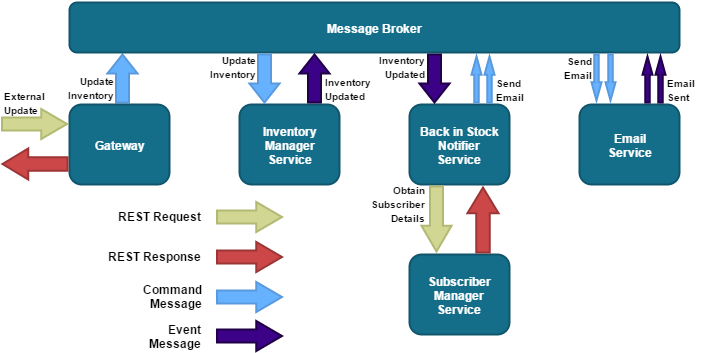
\includegraphics[width=80mm, height=50mm, scale=2]{img/mq-flow.png}
				\caption{Asynchronous calls}
			\end{figure}
		
		\vspace{5mm}
		\tiny {https://capgemini.github.io/architecture/is-rest-best-microservices}
	\end{frame}

	\begin{frame}
		\frametitle{Why not SOAP?}
				It is possible to build a microservices-based architecture using SOAP which uses HTTP. But:
			
			\vspace{5mm}
			\begin{itemize}
				\item
					\scriptsize {it only uses POST messages to transfer data to a server}.
					
				\item 
					\scriptsize{SOAP lacks concepts such as HATEOAS that enable relationships between microservices to be handled flexibly}. 
				\item 
					\scriptsize{The interfaces have to be completely defined by the server and known on the client}.
			\end{itemize}
			
			\vspace{30mm}
			\tiny {Microservices; Flexible Software Architecture. "Eberhard Wolff"}
	\end{frame}

	\subsection {API Gateway}
		\begin{frame}
		\frametitle{API Gateway}
			\begin{block} {API Gateway}
				\scriptsize {API Gateway is a tool that makes it easy for developers to create(1), publish(2), maintain(3), monitor(4), and secure(5) APIs at any scale. APIs act as the "front door" for applications to access data, business logic, or functionality from your backend services}.
			\end{block}
			\begin{figure}[h]
				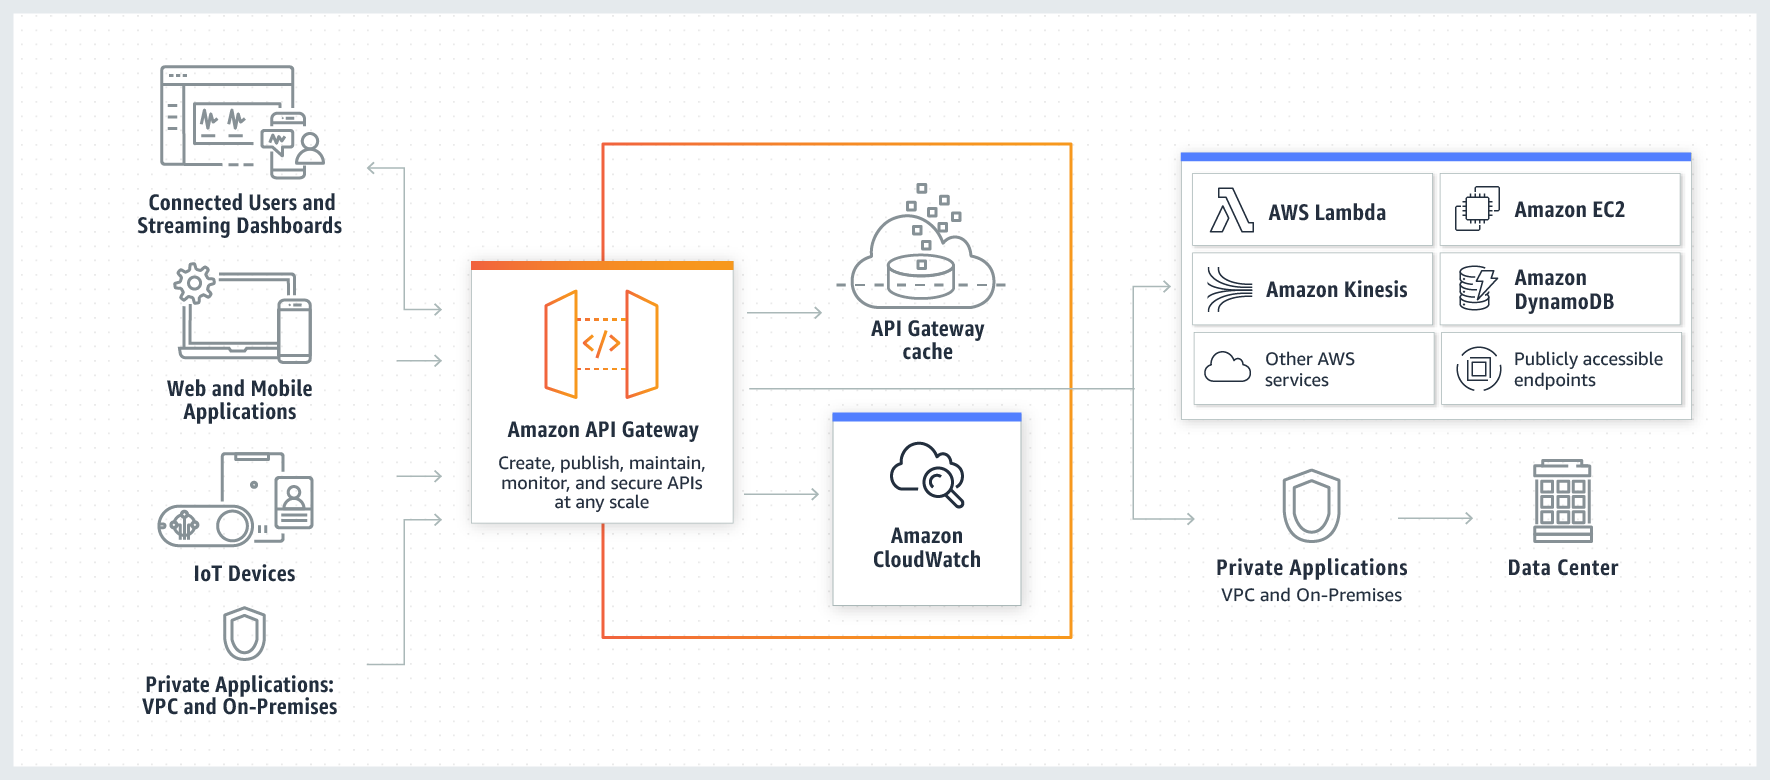
\includegraphics[width=100mm, scale=1]{img/amazon-gateway.png}
				\caption{Amazon Gateway}
			\end{figure}\vspace{1mm}
		
			\tiny{https://aws.amazon.com/api-gateway/}	
		\end{frame}
	
		\begin{frame}
			\frametitle{Orchestration and API Gateway cont...}
				\begin{figure}[h]
					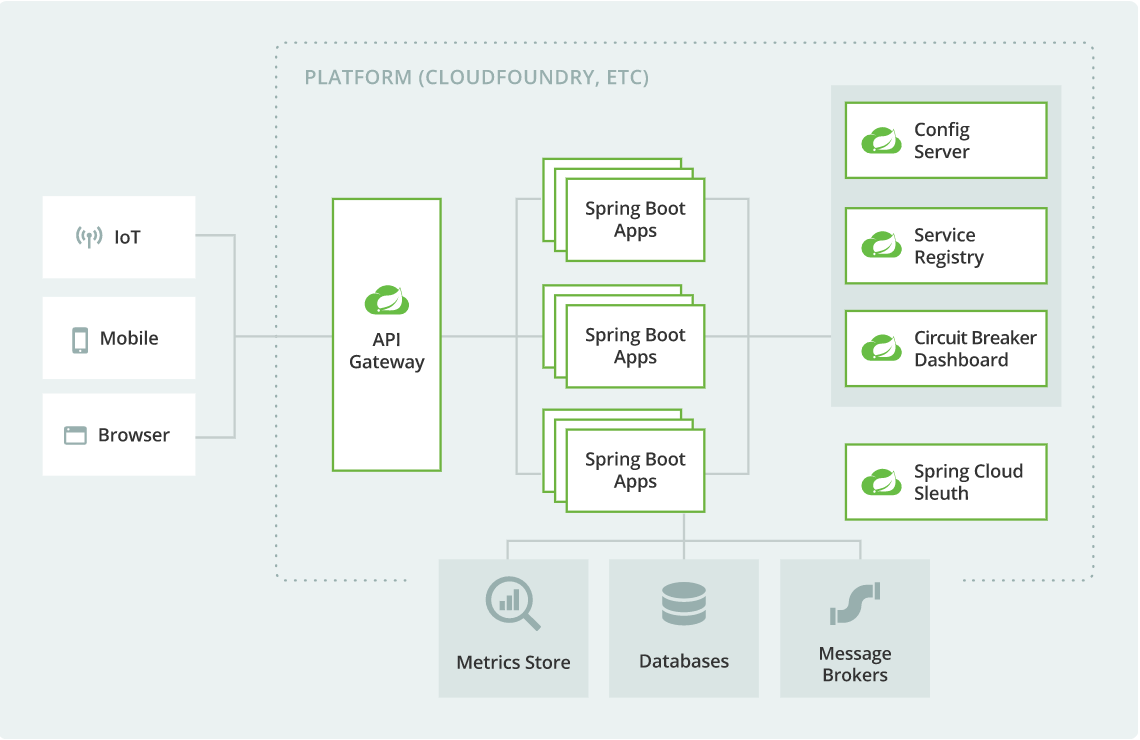
\includegraphics[width=100mm, scale=2]{img/microservice-diagrame.png}
					\caption{Microservices with Spring Cloud}
				\end{figure}\vspace{20mm}
				
				\tiny{https://spring.io/microservices}	
		\end{frame}
	
		\begin{frame}
			\frametitle{Available Market Options}
			\vspace{10mm}
				\begin{figure}[h]
					
\includegraphics[width=100mm, scale=2]{img/gtws.png}
					\caption{API Gateway Products}
				\end{figure}\vspace{20mm}
			
	\end{frame}
		
	
	
	\subsection {Service Discovery}
		\begin{frame}
			\frametitle{Service Discovery}
				\textbf {Problem} \par
					\small {In any distributed architecture, we need to find the physical address of where a machine is located}.
				
				\vspace{2mm}
				\textbf {Solution} \par	
					Using service discovery, a service can register itself when it is up and healthy. By using such technology you can achieve: 
						\begin{enumerate}
							\item<1->	Load balanced
								\begin{itemize}
									\item \scriptsize {dynamically load balance requests across all service instances to ensure that the service invocations are spread across all the service instances managed by it.}
								\end{itemize}
							\item<2-> 	Resilient
								\begin{itemize}
									\item \scriptsize {client should “cache” service information locally. Local caching allows for gradual 		degradation of the service discovery feature so that if service discovery service does become unavailable, applications can still function and locate the services based on the information maintained in its local cache.}
								\end{itemize}
							\item<3->	Fault-tolerant
								\begin{itemize}
									\item \scriptsize {detect when a service instance isn’t healthy and remove the instance from the list of available services.}
								\end{itemize}
							
						\end{enumerate}
			\vspace{10mm}
			\tiny{Spring Microservices in Action, ``JOHN CARNELL``}	
		\end{frame}
		
		\begin{frame}
		\frametitle{Service Discovery with Gateway}
			\begin{figure}[h]
				\centering
				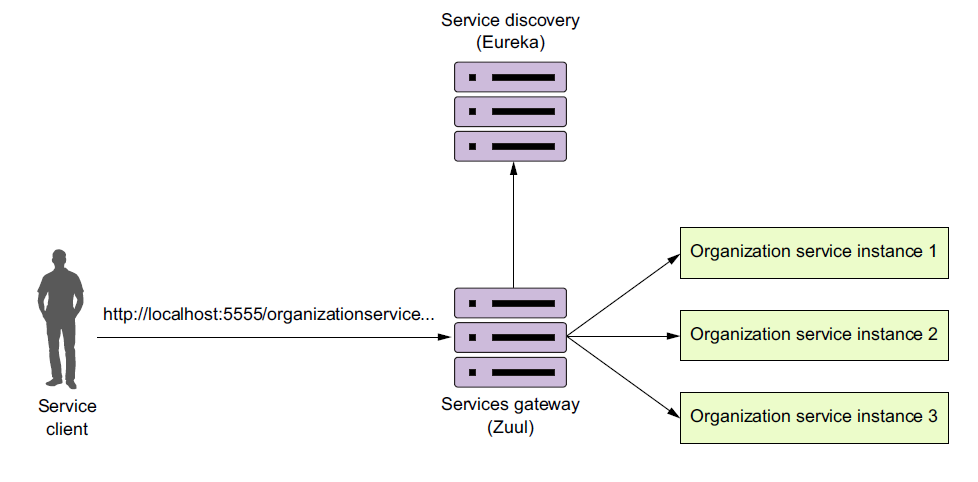
\includegraphics[width=.8\linewidth]{img/zull-and-sd.png}
				\caption{Service Registry and Gateway}
			\end{figure}
		\vspace{10mm}
		\tiny{Spring Microservices in Action, ``JOHN CARNELL``}	
		\end{frame}
		
		\begin{frame}
			\frametitle{Available Market Options}
				\begin{figure}[h]
						\centering
						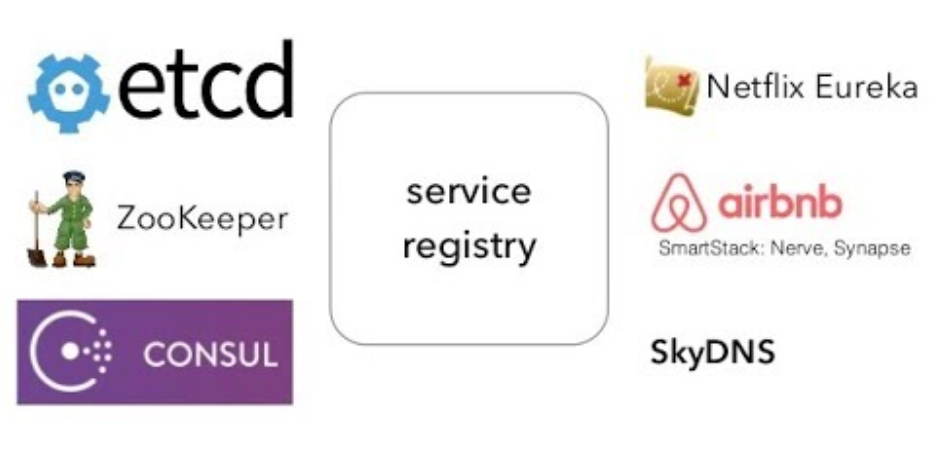
\includegraphics[width=.8\linewidth]{img/SR.png}
						\caption{Service Registry Products}
				\end{figure}
		\end{frame}
	
	\begin{frame}
		\frametitle{The Twelve-Factor App}
			The Twelve-Factor App methodology is a methodology for building \textbf{software-as-a-service} applications
			\begin{columns}[c]
				\column{.50\textwidth} 
				\begin{enumerate}
					\item Codebase
					\item Dependencies
					\item Config
					\item Backing services
					\item Build, release, run
					\item Processes
				\end{enumerate}
				
				\column{.50\textwidth} % Right column and width
				\begin{enumerate}
					\setcounter{enumi}{6}
					\item Port binding
					\item Concurrency
					\item Disposability
					\item Dev/prod parity
					\item Logs
					\item Admin processes
				\end{enumerate}
				
			\end{columns}
			\vspace{20mm}
			\tiny{https://12factor.net}	
		\end{frame}
	
		\begin{frame}
			\frametitle{The Twelve-Factor App}
				\begin{enumerate}
					\item Codebase
						\begin{itemize}
							\item One codebase tracked in revision control, many deploys
						\end{itemize}
				\end{enumerate}
				\begin{figure}[h]
					\centering
					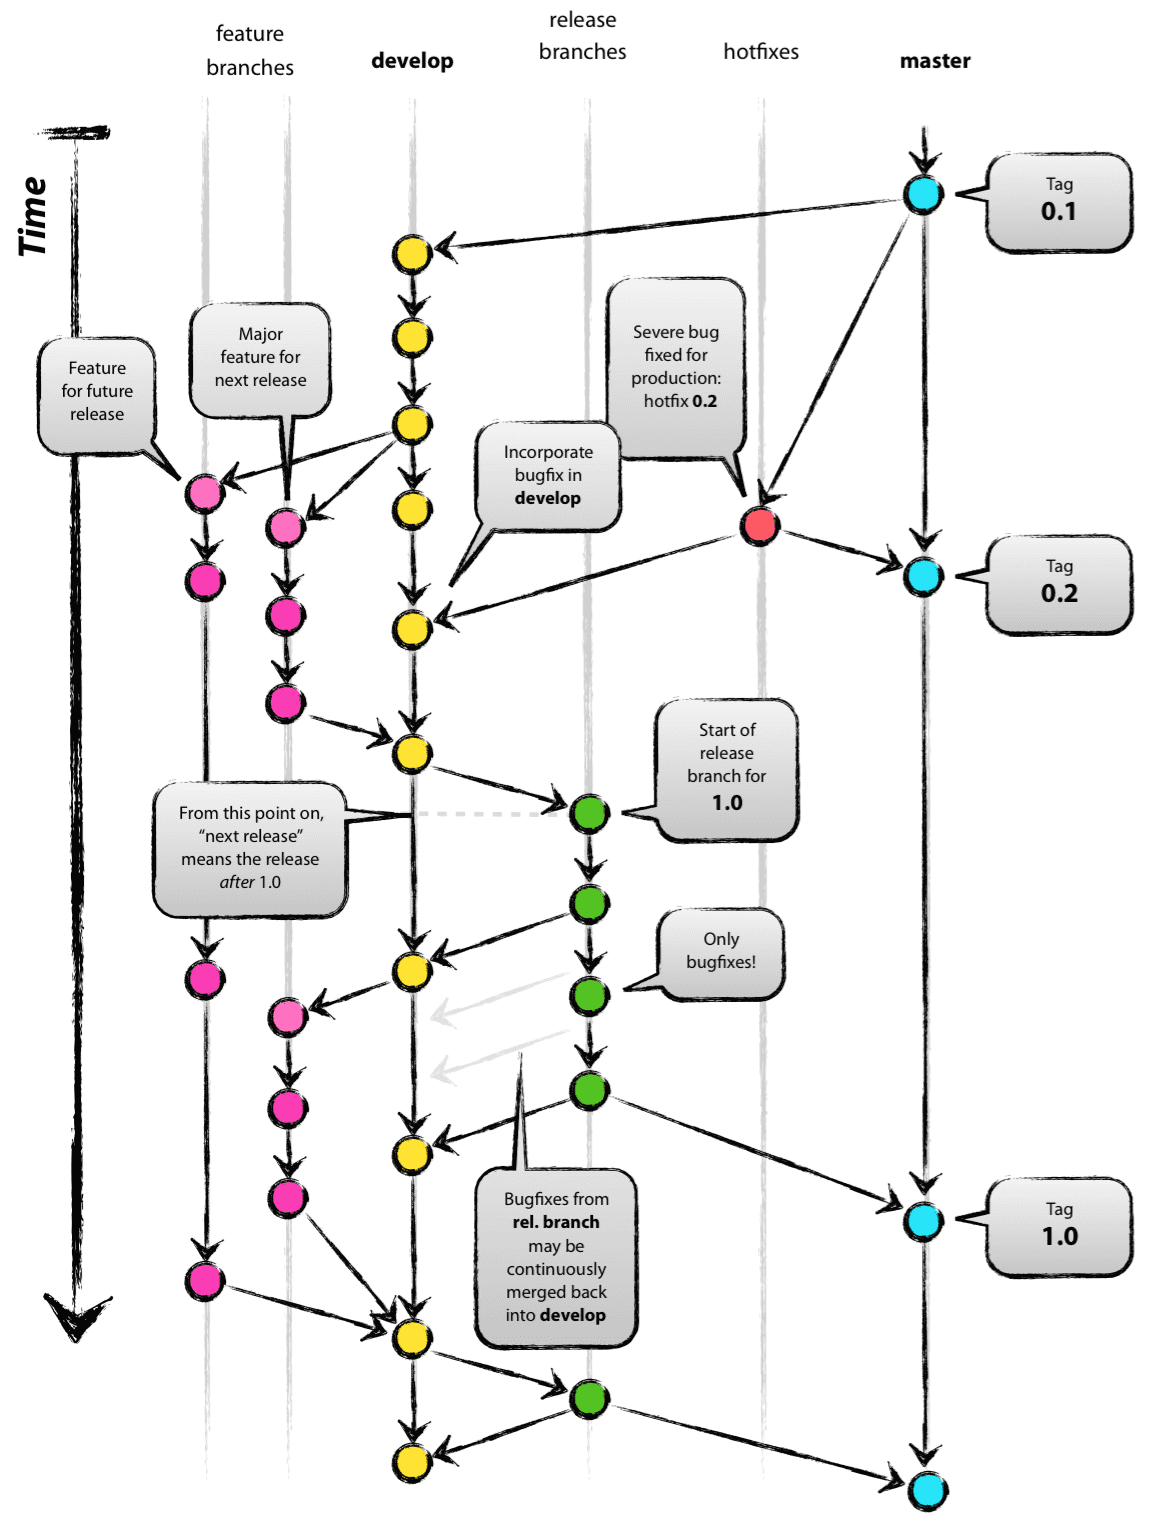
\includegraphics[width=.8\linewidth, height=65mm]{img/gitflow.png}
				\end{figure}
		\end{frame}
	
	\begin{frame}
		\frametitle{The Twelve-Factor App}
		\begin{enumerate}
			\setcounter{enumi}{1}
			\item Dependencies
			\begin{itemize}
				\item Explicitly declare and isolate dependencies
				\item Consider the magic key \textbf {Portability}
			\end{itemize}
		\end{enumerate}
		
		\begin{columns}[c]
			\column{.55\textwidth} 
				\begin{figure}[h]
					\centering
					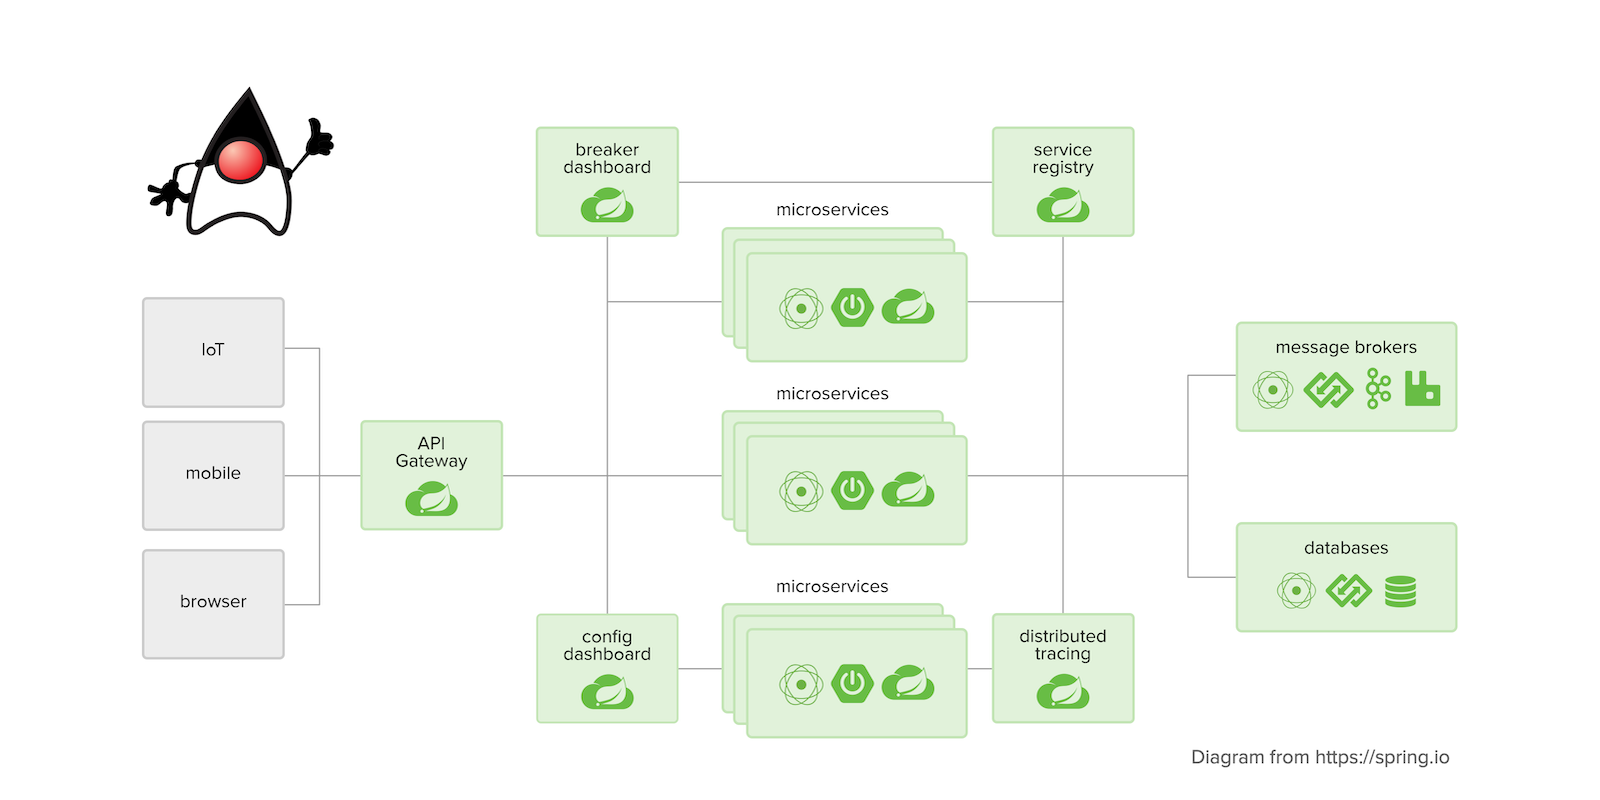
\includegraphics[width=1\linewidth, height=50mm, scale=1]{img/dpnc1.png}
				\end{figure}
			\column{.45\textwidth} % Right column and width
				\begin{figure}[h]
					\centering
					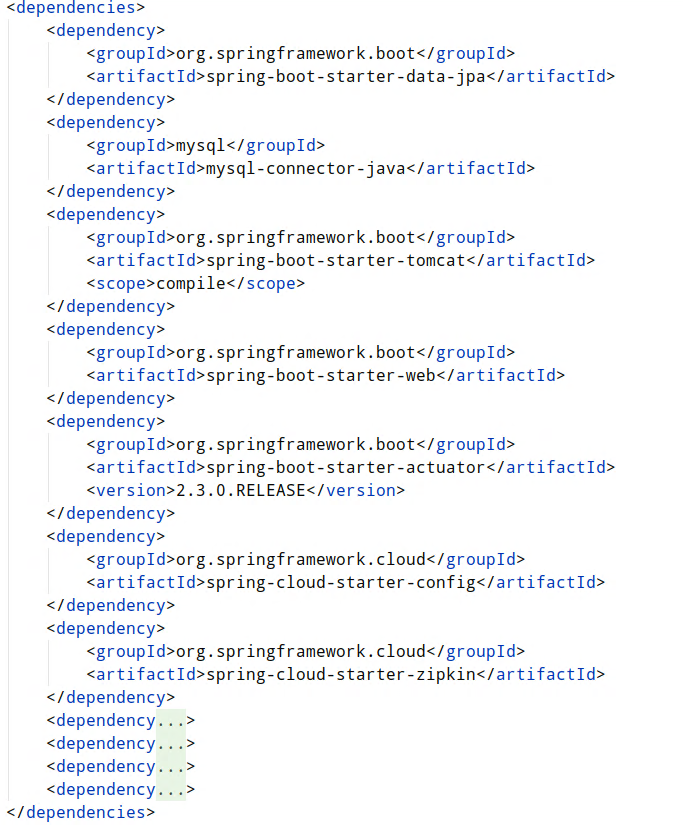
\includegraphics[width=1\linewidth, height=50mm, scale=1]{img/dpnc2.png}
				\end{figure}
			\end{columns}
		
		\vspace{4mm}
		\hspace{5mm} \textit {\color{red} Never ever depend on operating system}
		\vspace{26mm}
	\end{frame}
	
	\begin{frame}
	\frametitle{The Twelve-Factor App}
		\begin{enumerate}
			\setcounter{enumi}{2}
			\item Configuration
			\begin{itemize}
				\item<1-> Config is what is changed from environment to another
				\item<2-> Config should be provided by the environment, not the code
				
				\vspace{5mm}
				\item<3-> \textbf {Credentials are not configuration, but secrets}
				\begin{itemize}
					\item Never ever store credentials in code
					\item Don't save credentials in PLAINTEXT with config, but hashed
				\end{itemize}
				
				\vspace{5mm}
				\item<4-> \textbf {Configuration in Legacy system is a challenge}
				\begin{itemize}
					\item Unlike missing dependencies, System will not immediately crashed if configuration is missed
					\item Give attention to URLs in legacy code
				\end{itemize}
			\end{itemize}
		\end{enumerate}
	\vspace{30mm}
	\end{frame}
	

	\subsection {Externalized Configurations}
		\begin{frame}
			\frametitle{Externalized and \color{green} {Dynamic Configurations}}
				\textbf {Problem} \par
					\hspace{3mm}\small {Configurations will vary from environment to another, How to manage them?}
				
				\vspace{2mm}
				\textbf {Solution} \par	
					\hspace{3mm}\small {Centralize your configuration} 
				
				\begin{figure}[h]
					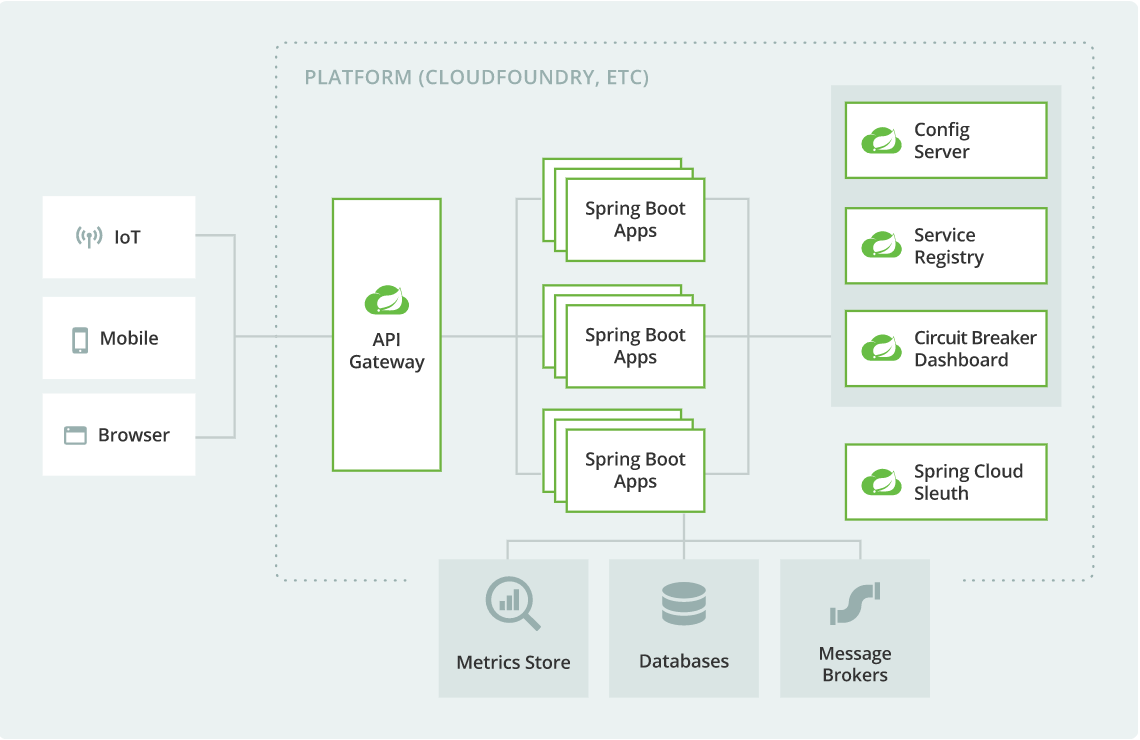
\includegraphics[width=100mm,height=50mm, scale=1]{img/microservice-diagrame.png}
					\caption{Microservices with Spring Cloud}
				\end{figure}\vspace{20mm}
				
				\tiny{https://spring.io/microservices}	
		\end{frame}
	
	\begin{frame}
		\frametitle{Available Market Options}
			
			\begin{figure}[h]
				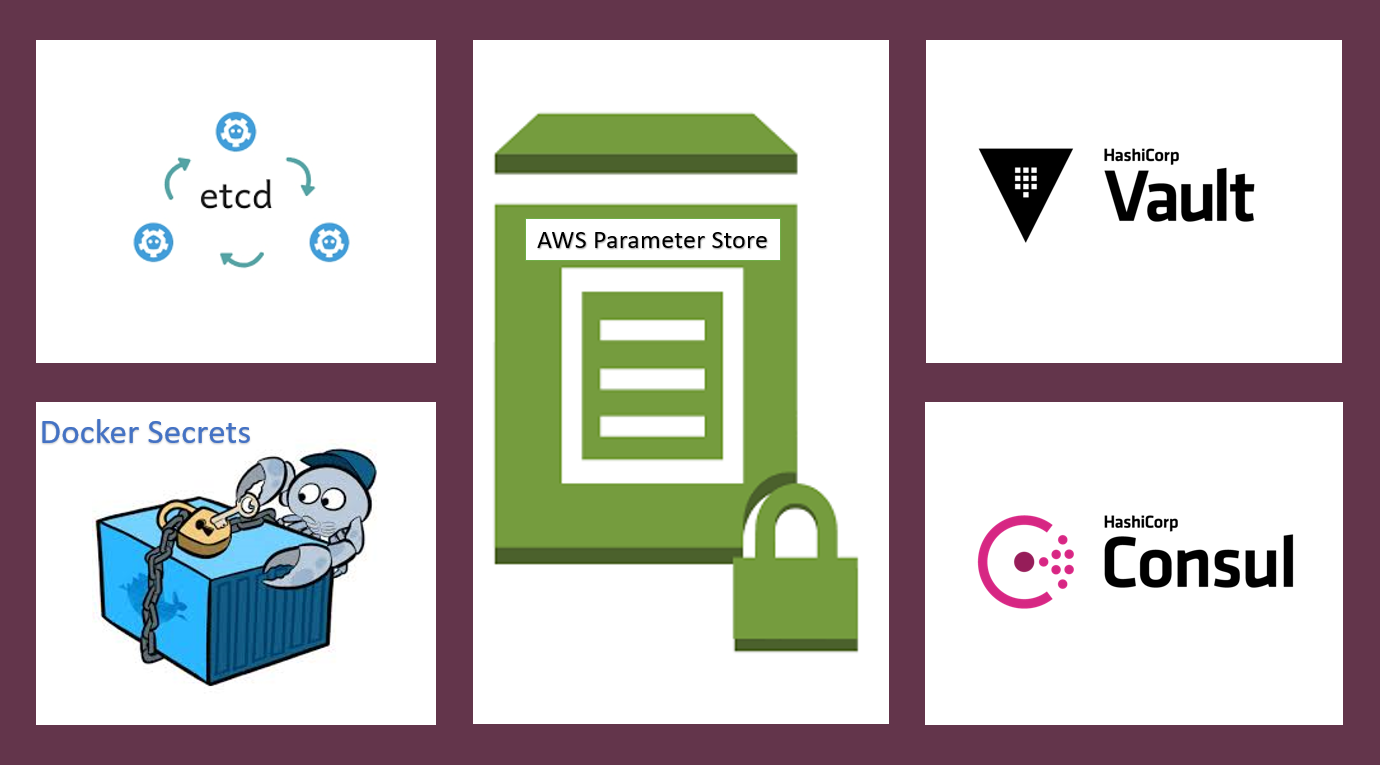
\includegraphics[width=100mm,height=60mm,  scale=1]{img/Configs.png}
				\caption{Popular Config Stores}
			\end{figure}\vspace{20mm}
			
			\tiny{https://spring.io/microservices}	
	\end{frame}

	\subsection {Circuit Breaker Pattern}
		\begin{frame}
			\frametitle{Circuit Breaker Pattern}
			\textbf {Problem} \par
			\begin{itemize}
				\item<1-> \scriptsize {One of the big differences between in-memory calls and remote calls is that remote calls can fail, or hang without a response until some timeout limit is reached}.
				\item<2-> \scriptsize {What's worse if you have many callers on a unresponsive supplier, then you can run out of critical resources leading to cascading failures across multiple systems}.
			\end{itemize}  
			\textbf {Solution} \par
			\hspace{3mm} \small {Fault Tolerance}
			\begin{figure}[h]
				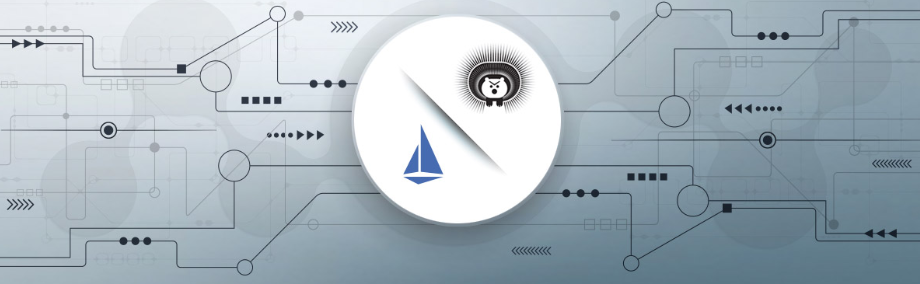
\includegraphics[width=100mm,scale=1]{img/cbp.png}
				\caption{Circuit Breaker}
			\end{figure}\vspace{20mm}
		
			\tiny{https://www.exoscale.com/syslog/istio-vs-hystrix-circuit-breaker/}	
		\end{frame}
	
	
		\begin{frame}
			\frametitle{The Twelve-Factor App}
				\begin{enumerate}
					\setcounter{enumi}{3}
					\item Backing Service \\
						\begin{itemize}
							\item A backing service is any service the app consumes over the network as part of its normal operation. 
							\item Examples include data stores, queueing, and caching systems
						\end{itemize}
						\vspace{2mm}
				\end{enumerate}
			\vspace{100mm}
		\end{frame}
	
		\begin{frame}
			\frametitle{The Twelve-Factor App}
				\begin{enumerate}
					\setcounter{enumi}{3}
					\item Backing Service \\
					\begin{itemize}
						\item A backing service is any service the app consumes over the network as part of its normal operation. 
						\item Examples include data stores, queueing, and caching systems
					\end{itemize}
					\vspace{2mm}
					
					\hspace{2mm} How to achieve that?\\
					\begin{itemize}
						\item<1-> \scriptsize {To the App, this is just normal service}.
						\item<2-> \scriptsize {Should be treating as \textbf {attached resource}}.
						\item<3-> \scriptsize {Even with third party services like SMTP providers, it is just a resource}.
						\item<4-> \scriptsize {A good way for this is as mentioned in config talk}.\\
							\lstinputlisting[language=Java]{attch-resource.java}
						\item<5-> \small {\color{blue}{This way you can switch between services smoothly on different environments via configurations provided by the environment}}.
					\end{itemize}
				\end{enumerate}
			\vspace{100mm}
		\end{frame}
		
		
		\begin{frame}
			\frametitle{Development Culture}
				Usually building a microservices software requires good development strategy to follow, and the most valuable one is \\
				\vspace{100mm}
		\end{frame}
	
		\begin{frame}
			\frametitle{Development Culture}
			Usually building a microservices software requires good development strategy to follow, and the most valuable one is \\
			
			\vspace{1mm}
			\hspace{3mm} \textbf {Agile} \\
			
			\begin{enumerate}
				\item<1-> \scriptsize {Working in small planned sprints period}
				\item<2-> \scriptsize {Each sprint is 2 to 4 weeks} 
				\item<3-> \scriptsize {Stand-up meeting for 15 mins to discuss challenges and day to day work}
				\item<4-> \scriptsize {Feedback and Retrospective meetings after each sprint is very important}
			\end{enumerate}
		
			\begin{figure}[h]
				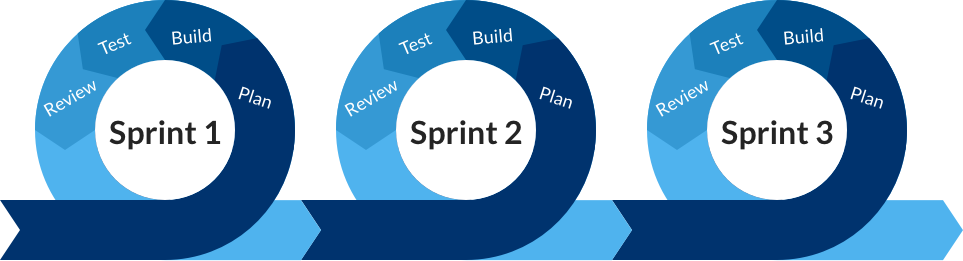
\includegraphics[width=100mm,scale=1]{img/agile.png}
				\caption{Agile Methodology}
			\end{figure}
		\end{frame}
		
		\begin{frame}[label=ci]
			\frametitle{The Twelve-Factor App}
				\begin{enumerate}
					\setcounter{enumi}{4}
					\item Build, Release and Run (CI \& CD) \\
					\small {Strictly separate build and run stages. In Microservices, this process is always related directly to development culture; How to be sure each time work will be delivered correctly?}\\
				\end{enumerate}
			
			\begin{figure}[h]
				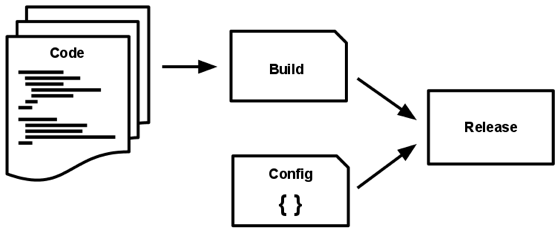
\includegraphics[width=100mm,scale=1]{img/release.png}
			\end{figure}
		\end{frame}
		
		\begin{frame}
		\frametitle{The Twelve-Factor App}
			\begin{enumerate}
				\setcounter{enumi}{4}
				\item Build, Release and Run (CI \& CD) \\
				\vspace{2mm}
				\begin{itemize}
					\item {Build}
						\begin{itemize}
							\item<1-> \scriptsize {The process where you convert the code into executable bundles}.
							\vspace{2mm}
							\item<2-> \scriptsize {Each build should be correct, and to achieve that, you have to use Continues Integration flow}.\vspace{2mm}
							\item<3-> \scriptsize {Each team member must write the unit and integration tests which will be executed before and after the build}.\vspace{2mm}
							\item<4-> \scriptsize {Tests which are written, must be strictly reviewed}.
							\vspace{2mm}
							\item<5-> \scriptsize {It is nice today to use TDD while developing to gain more experience and understanding}.
							\vspace{2mm}
							\item<6-> \scriptsize {\color{red} Don’t Comment Out Failing Tests}
							\vspace{2mm}
							\item<7-> \scriptsize {\color{red} Don't push broken code}.
						\end{itemize}
				\end{itemize}
			\end{enumerate}
		\vspace{20mm}
		\tiny{Continuous Delivery, ``JEZ HUMBLE`` \& ``DEVID FARLEY``}	
		\end{frame}
	
		\begin{frame}
		\frametitle{The Twelve-Factor App}
			\begin{enumerate}
				\setcounter{enumi}{4}
				\item Build, Release and Run (CI \& CD) \\
				\vspace{2mm}
				\begin{itemize}
					\item {Build}
					\begin{figure}[h]
						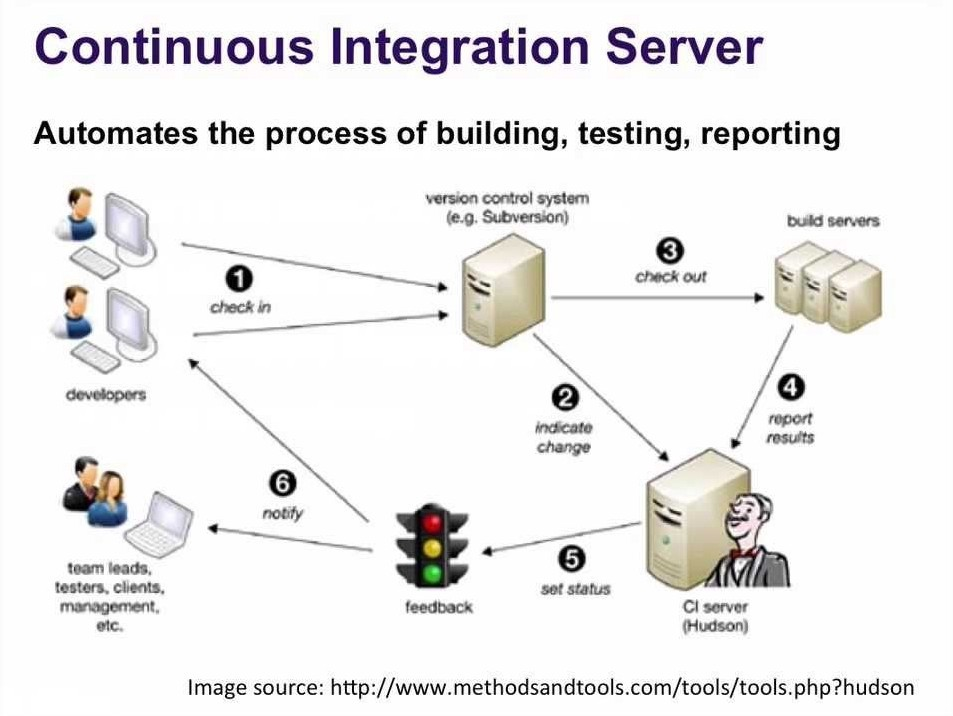
\includegraphics[width=100mm,height= 60mm, scale=1]{img/ci.jpeg}
						\caption{CI Workflow}
					\end{figure}
				\end{itemize}
			\end{enumerate}
		\end{frame}
	
		\begin{frame}
			\frametitle{The Twelve-Factor App}
				\begin{enumerate}
					\setcounter{enumi}{4}
					\item Build, Release and Run (CI \& CD) \\
					\vspace{2mm}
					\begin{itemize}
						\item {Release}
						\begin{itemize}
							\item<1-> \scriptsize {The process where you combine the build with deploy's config}.\vspace{2mm}
							\item<2-> \scriptsize {If the tests passed , build stage is done; and move to release stage}.\vspace{2mm}
							\item<3-> \scriptsize {The resulting release contains both the build and the config and is ready for immediate execution in the execution environment}.\vspace{2mm}
							\item<4-> \scriptsize {Every release should always have a unique release ID, such as a timestamp of the release (such as 2011-04-06-20:32:17) or an incrementing number (such as v100)}.\vspace{2mm}
							\item<5-> \scriptsize {Release are immutable, any change should be mapped with a new release}.\vspace{2mm}
							\item<6-> \scriptsize {Using tagging, unique IDs and timestamp will be the only way to apply rollback if you want}.
						\end{itemize}
					\end{itemize}
				\end{enumerate}
		\end{frame}
	
		\begin{frame}
		\frametitle{The Twelve-Factor App}
			\begin{enumerate}
				\setcounter{enumi}{4}
				\item Build, Release and Run (CI \& CD) \\
				\vspace{2mm}
				\begin{itemize}
					\item {Run}
					\begin{itemize}
						\item<1-> \scriptsize {also known as “runtime”, runs the app in the execution environment, by launching some set of the app’s processes against a selected release}.\vspace{2mm}
						
						\item<2-> \scriptsize {Builds are initiated by the app’s developers whenever new code is deployed. Runtime execution, by contrast, can happen automatically in cases such as a server reboot, or a crashed process being restarted by the process manager}. \vspace{2mm}
						
						\item<3-> \scriptsize {the run stage should be kept to as few moving parts as possible, since problems that prevent an app from running can cause it to break in the middle of the night when no developers are on hand.}
					\end{itemize}
				\end{itemize}
			\end{enumerate}
		\end{frame}

	\againframe{ci}
	
	\begin{frame}
		\frametitle{The Twelve-Factor App}
			\begin{enumerate}
				\setcounter{enumi}{5}
				\item Processes \\
				\hspace{2mm} \small{Execute the app as one or more \textbf{stateless} processes}
				\vspace{2mm}
				\begin{itemize}
					\item<1-> \scriptsize {Twelve-factor processes are stateless and share-nothing, and indeed Microservices are the same.}
					\vspace{2mm}
					\item<2-> \scriptsize {Any data that needs to persist must be stored in a stateful backing service, typically a database.}
					\vspace{2mm}
					\item<3-> \scriptsize {Asset packagers like \textit{django-assetpackager} use the filesystem as a cache for compiled assets. This process of compiling should be done during the \textbf{build} stage.}
					\vspace{2mm}
					\item<4-> \scriptsize {For example, using filesystems and caching memory is a violation of twelve factor.}
					\vspace{2mm}
					\item<5-> \scriptsize {Session state data is a good candidate for a datastore that offers time-expiration, such as Memcached or Redis.}
					\vspace{2mm}
					\item<6-> \scriptsize {It is important to know also that, Microservices must be totally stateless, and there is no way to keep state for backend services http requests.}
				\end{itemize}
			\end{enumerate}
		\vspace{20mm}
	\end{frame}
	
	\begin{frame}
		\frametitle{The Twelve-Factor App}
		\begin{enumerate}
			\setcounter{enumi}{6}
			\item Port Binding \\
			\hspace{2mm} \scriptsize{Export services via port binding}
		\end{enumerate}
		\vspace{100mm}
	\end{frame}

	\begin{frame}
		\frametitle{The Twelve-Factor App}
			\begin{enumerate}
				\setcounter{enumi}{6}
				\item Port Binding \\
				\hspace{2mm} \scriptsize{Export services via port binding}
				\vspace{1mm}
				\begin{itemize}
					\item<1-> \scriptsize {The Microservice is self-contained and does not rely on injection of a webserver to create a web-facing service.}
					\item<2-> \scriptsize {In a local development environment, you can visit a service URL like http://localhost:5000/ to access the service exported by their app.}
					\item<3-> \scriptsize {In deployment, a routing layer handles routing requests from a public-facing hostname to the port-bound web processes.}
				\end{itemize}
			\end{enumerate}
			\begin{figure}[h]
				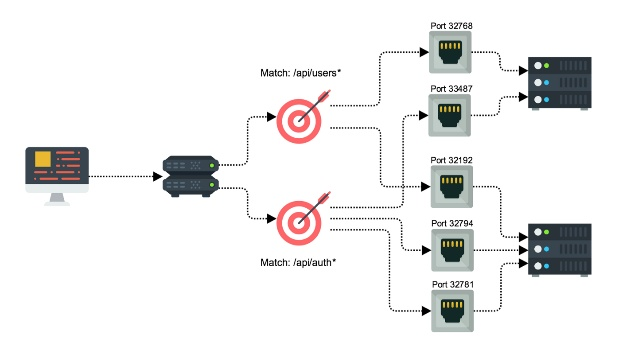
\includegraphics[width=100mm,height= 50mm, scale=1]{img/port-binding.jpg}
			\end{figure}
	\end{frame}

	\subsection {Data Sharing and Management}
		\begin{frame}
			\frametitle{Data Sharing and Management}
				In old monilithic style, life was someway easy, but with microservices data management; you need to play harder.
				
				\begin{figure}[h]
					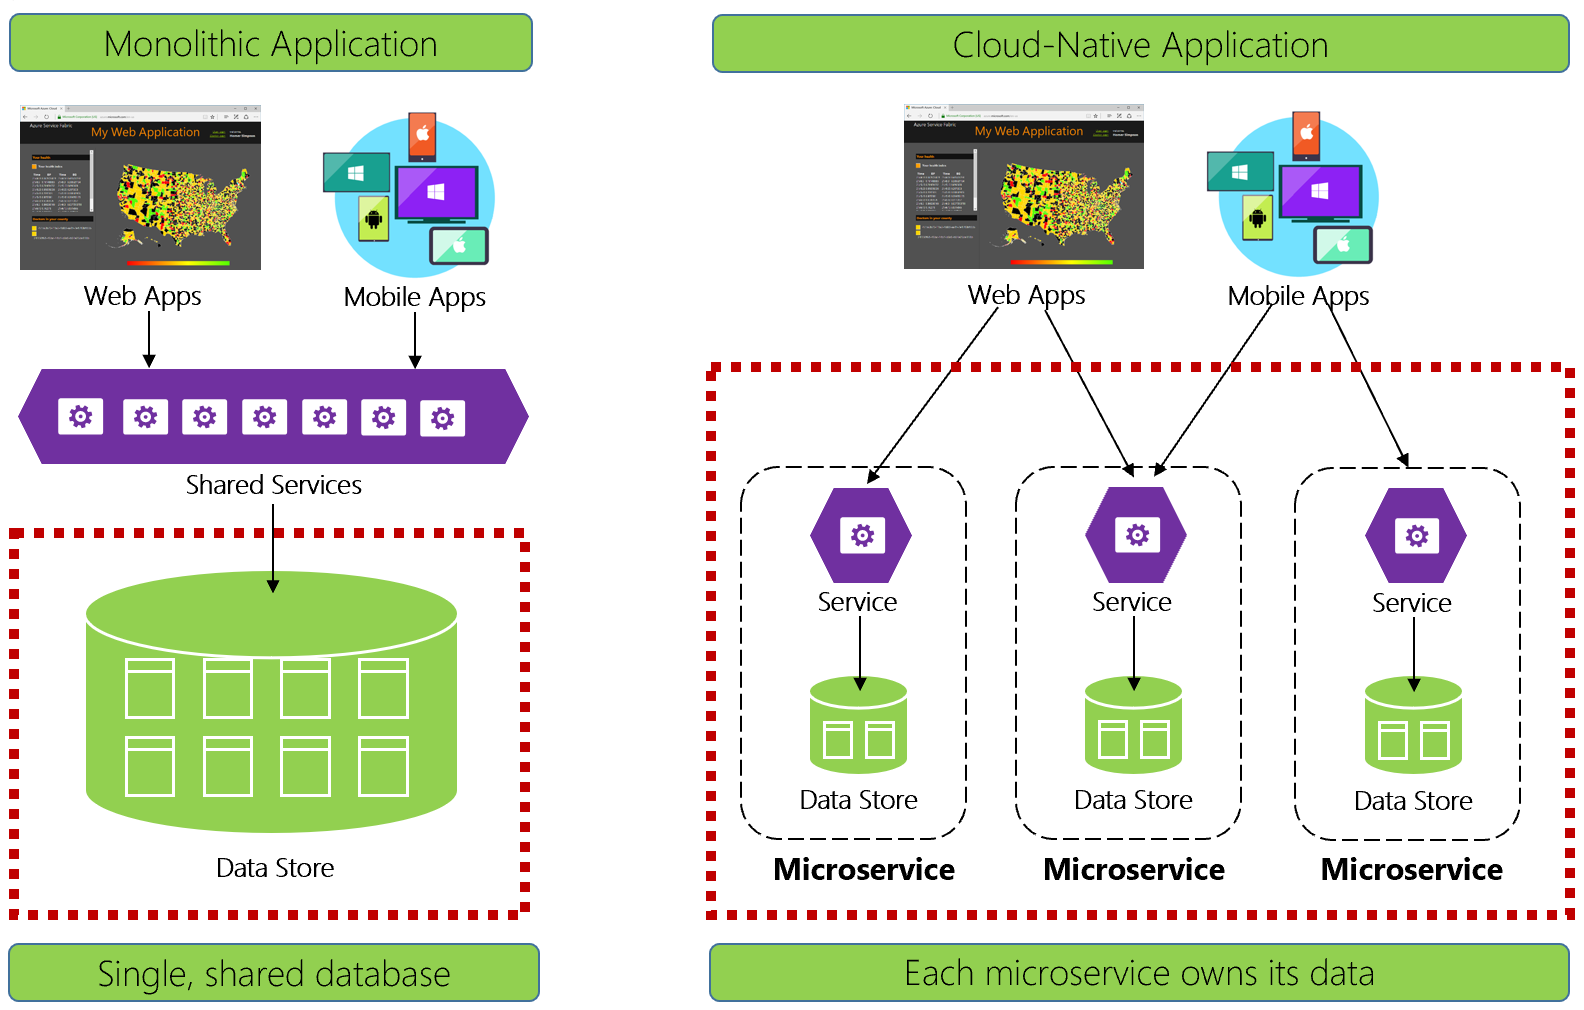
\includegraphics[width=100mm,height= 50mm, scale=1]{img/distributed-data.png}
					\caption{Distributed Data Architecture}
				\end{figure}
			\tiny{https://docs.microsoft.com/en-us/dotnet/architecture/cloud-native/distributed-data}	
		\end{frame}
	
		\begin{frame}
			\frametitle{Data Sharing and Management}
				Why database per service?
					\begin{itemize}
						\item<1-> \scriptsize{Domain data is encapsulated within the service }
						\item<2-> \scriptsize{Data schema can evolve without directly impacting other services code and functionality}
						\item<3-> \scriptsize{Each data store can independently scale}
						\item<4-> \scriptsize{Data store failure in one service won't directly impact other services}
					\end{itemize}
				\vspace{100mm}
		\end{frame}
	
		\begin{frame}
			\frametitle{Data Sharing and Management}
				Why database per service?
				\begin{itemize}
					\item \scriptsize{Domain data is encapsulated within the service }
					\item \scriptsize{Data schema can evolve without directly impacting other services code and functionality}
					\item \scriptsize{Each data store can independently scale}
					\item \scriptsize{Data store failure in one service won't directly impact other services}
				\end{itemize}
				
				\vspace{5mm}
				\textbf{BUT}\\
				\hspace{3mm} \scriptsize{You can also use single DB server and achieve some sort of that, How?} 
				\vspace{100mm}
			\end{frame}
		
		\begin{frame}
			\frametitle{Data Sharing and Management}
				Why database per service?
				\begin{itemize}
					\item \scriptsize{Domain data is encapsulated within the service }
					\item \scriptsize{Data schema can evolve without directly impacting other services code and functionality}
					\item \scriptsize{Each data store can independently scale}
					\item \scriptsize{Data store failure in one service won't directly impact other services}
				\end{itemize}
				
				\vspace{5mm}
				\textbf{BUT}\\
				\hspace{3mm} \scriptsize{You can also use single DB server and achieve some sort of that, How?} 
				\begin{itemize}
					\item<1-> \scriptsize{Schema management; that is each service has its own schema}
					\item<2-> \scriptsize{Tables' access privilege}
					\item<3-> \scriptsize{Database readonly views }
				\end{itemize}
				\vspace{100mm}
			\end{frame}
		
		\begin{frame}
		\frametitle{Data Sharing and Management}
			Why database per service?
			\begin{itemize}
				\item \scriptsize{Domain data is encapsulated within the service }
				\item \scriptsize{Data schema can evolve without directly impacting other services code and functionality}
				\item \scriptsize{Each data store can independently scale}
				\item \scriptsize{Data store failure in one service won't directly impact other services}
			\end{itemize}
			
			\vspace{5mm}
			\textbf{BUT}\\
			\hspace{3mm} \scriptsize{You can also use single DB server and achieve some sort of that, How?}
			\begin{itemize}
				\item \scriptsize{Schema management; that is each service has its own schema}
				\item \scriptsize{Tables' access privilege}
				\item \scriptsize{Database readonly views}
			\end{itemize}
		
			\vspace{5mm}
				Which way is better? \\
					\hspace{3mm} \scriptsize {A: It depends. However it is recommended to follow best practices}.\\
					\hspace{3mm} \scriptsize {The more simple and focused service you have, the easier management you get. A perfect way to do that, is applying DDD principles}.
			\vspace{100mm}
		\end{frame}
	
		\begin{frame}
			\frametitle{Data Sharing and Management}
			Why database per service?
			\begin{itemize}
				\item \scriptsize{Domain data is encapsulated within the service }
				\item \scriptsize{Data schema can evolve without directly impacting other services code and functionality}
				\item \scriptsize{Each data store can independently scale}
				\item \scriptsize{Data store failure in one service won't directly impact other services}
			\end{itemize}
			
			\vspace{5mm}
			\textbf{BUT}\\
			\hspace{3mm} \scriptsize{You can also use single DB server and achieve some sort of that, How?}
			\begin{itemize}
				\item \scriptsize{Schema management; that is each service has its own schema}
				\item \scriptsize{Tables' access privilege}
				\item \scriptsize{Database readonly views}
			\end{itemize}
			
			\vspace{5mm}
			Which way is better? \\
			\hspace{3mm} \scriptsize {A: It depends. However it is recommended to follow best practices}.\\
			\hspace{3mm} \scriptsize {The more simple and focused service you have, the easier management you get. A perfect way to do that, is applying DDD principles}.
			
			\vspace{2mm}
			\scriptsize{ \alert{While encapsulating data into separate microservices can increase agility, performance, and scalability, it also presents many challenges.}}
			\vspace{100mm}
		\end{frame}
	
	\begin{frame}
		\frametitle{Data Sharing and Management}
			Cross-Service Queries \\
			\vspace{1mm}
			\hspace{3mm} \scriptsize {Usually you need to integrate to get$\backslash$query data from other services}
			\begin{figure}[h]
				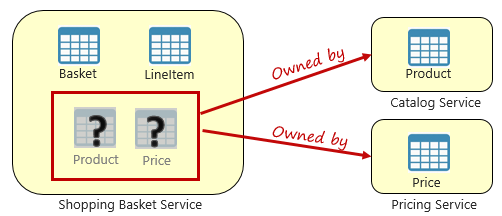
\includegraphics[width=100mm,height= 50mm, scale=1]{img/csq.png}
				\caption{Querying across microservices}
			\end{figure}
			\tiny{https://docs.microsoft.com/en-us/dotnet/architecture/cloud-native/distributed-data}	
			\vspace{100mm}
	\end{frame}

	\begin{frame}
		\frametitle{Data Sharing and Management}
		Cross-Service Queries \\
		\vspace{1mm}
		\hspace{3mm} \scriptsize {Usually you need to integrate to get$\backslash$query data from other services}
		\vspace{1mm}
			\begin{itemize}
				\item<1-> \scriptsize{First and easiest way is to query service's database directly, \alert{Anti-Pattern}}
				\item<2-> \scriptsize{Also another simple way is through HTTP, but this may leads to coupling issues}
				\item<3-> \scriptsize{Third option is using asynchronous calls via queues, and you should give attention to this}
				\item<4-> \scriptsize{If the data volume is huge, and is not changed quickly, good way to use is}
					\begin{figure}[h]
						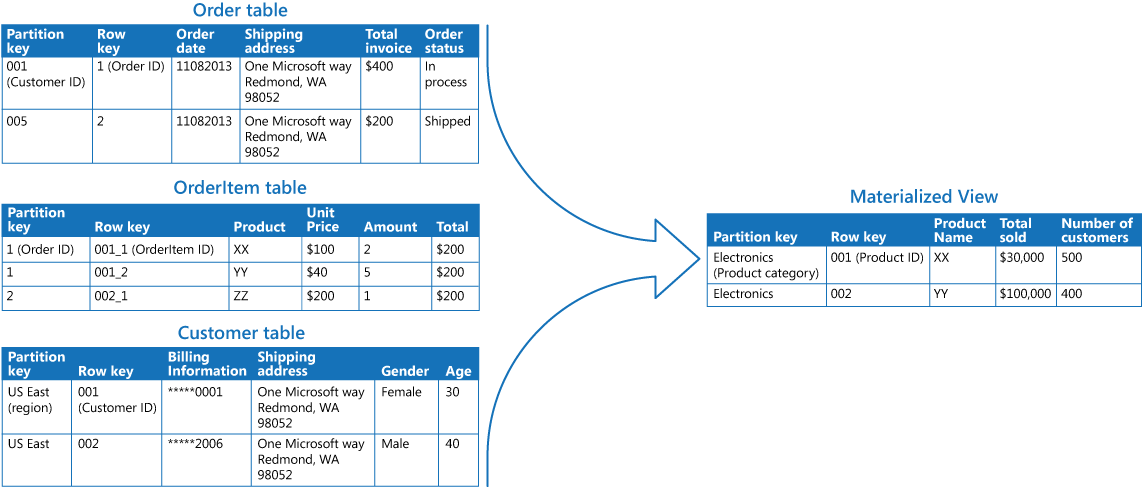
\includegraphics[width=100mm,height= 50mm, scale=1]{img/mat-view.png}
						\caption{Materialized Views Pattern}
					\end{figure}
			\end{itemize}
			
		\vspace{100mm}
	\end{frame}

	\begin{frame}
	\frametitle{Data Sharing and Management}
	Distributed Transactions \\
	\vspace{1mm}
	\hspace{3mm} \scriptsize {We move from a world of \textbf{immediate consistency} to that of \textbf{eventual consistency}}\\
	\hspace{3mm} \scriptsize {That is; in microservices. You can't depend on ACID transaction, but \\ 
		\hspace{3mm} \textbf{BASE} which is acronym for \textbf Basic \textbf Availability, \textbf Soft-state, and \textbf Eventual consistency}
	\vspace{1mm}
		\begin{figure}[h]
			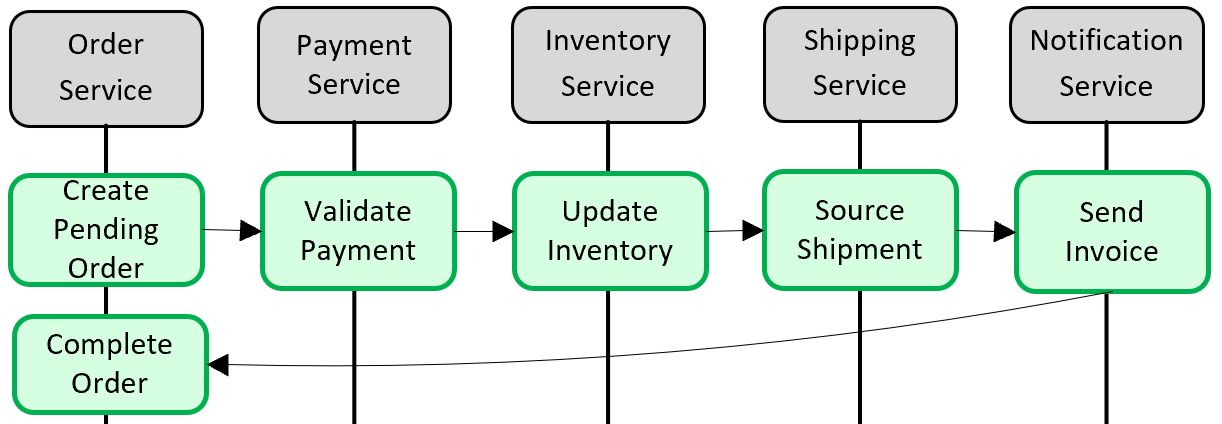
\includegraphics[width=100mm,height= 45mm, scale=1]{img/saga-tr.png}
			\caption{Transaction across microservices}
		\end{figure}
		\tiny{https://docs.microsoft.com/en-us/dotnet/architecture/cloud-native/distributed-data}
	\vspace{100mm}
	\end{frame}

	\begin{frame}
		\frametitle{Data Sharing and Management}
		Distributed Transactions \\
		\vspace{1mm}
			\begin{itemize}
				\item<1-> \scriptsize{Having multiple data sources on different zones will make consistency issue}
				\item<2-> \scriptsize{No options to handle that except Programmatic approach}
				\item<3-> \scriptsize{First available way is 2-Phase-commits \textbf{2PC}}
				\begin{figure}[h]
					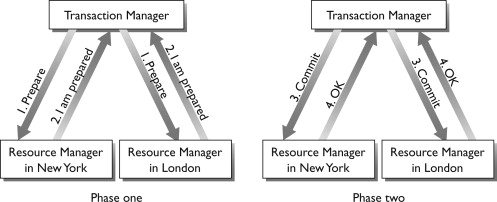
\includegraphics[width=100mm,height= 40mm, scale=1]{img/2pc.jpg}
					\caption{Two-phase Commit pattern}
				\end{figure}
			\item<4-> \scriptsize{\alert{In real case, this is impractical, and will lead to locking and time consuming issue}}
			\end{itemize}
		\vspace{5mm}
		\tiny{https://www.sciencedirect.com/topics/computer-science/two-phase-commit}
	\end{frame}

	\begin{frame}
		\frametitle{Data Sharing and Management}
		Distributed Transactions \\
		\vspace{1mm}
		\begin{itemize}
			\item<1-> \scriptsize{Having multiple data sources on different zones will make consistency issue}
			\item<1-> \scriptsize{No options to handle that except Programmatic approach}
			\item<1-> \scriptsize{First available way is 2-Phase-commits \textbf{2PC}}
			\item<2-> \scriptsize{Another approach; If moving from point to point is succeeded, continue; else \textbf{Compensate}}
			\item<3-> \scriptsize{The big father of this approach is \textbf{Saga pattern}}
				\begin{figure}[h]
					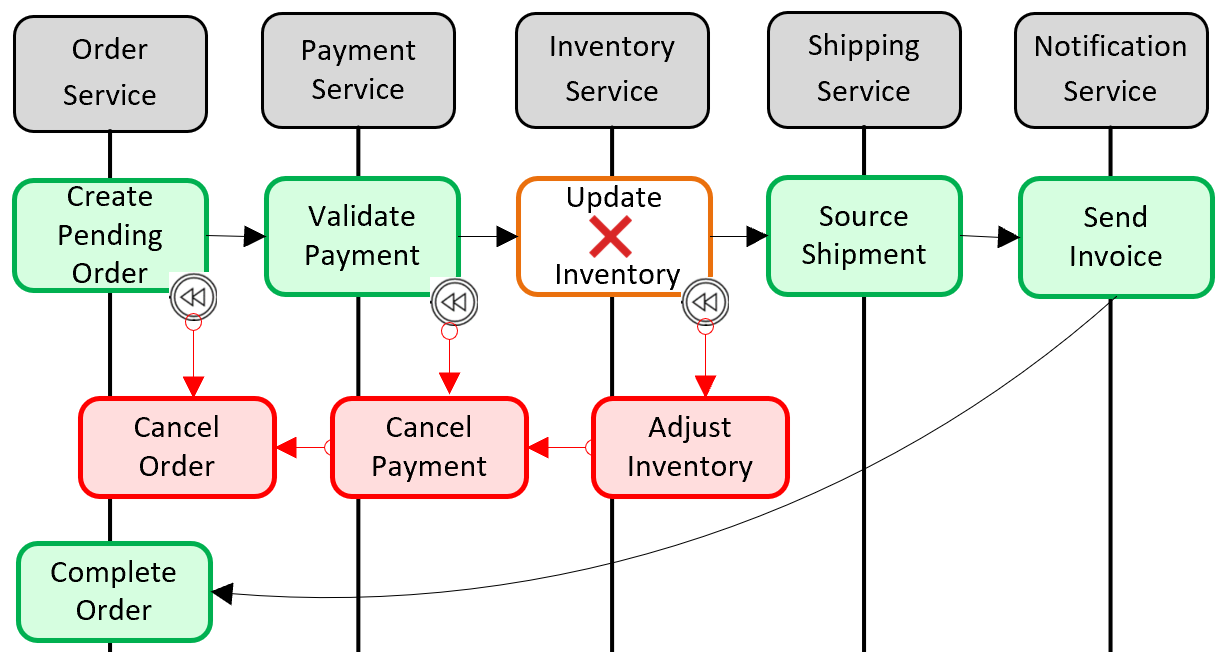
\includegraphics[width=100mm,height= 50mm, scale=1]{img/saga-rollback.png}
					\caption{Rolling back a transaction}
				\end{figure}
		\end{itemize}
	\end{frame}
	
	\begin{frame}
		\frametitle{Data Sharing and Management}
		Command and Query Responsibility Segregation (\textbf{CQRS})  
		\begin{itemize}
			\item<1->[] \small{Cloud native applications need sometimes to handle huge data.}
			\vspace{1mm}
			\item<2-> \scriptsize{In monolithic, there is no problem to handle this for simple CRUD operations}
			\item<3-> \scriptsize{Adding good managed indexes for example can solve the issue}
			\item<4-> \scriptsize{But read is not only the concern you focus on, but also writes}
			\item<2->[]
				\begin{figure}[h]
					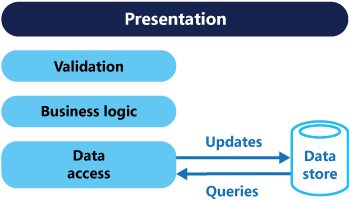
\includegraphics[width=75mm,height= 35mm, scale=1]{img/tradition-crud.png}
					\caption{Traditional Application Architecture}
				\end{figure}
		\end{itemize}
	\end{frame}


		\begin{frame}
		\frametitle{Data Sharing and Management}
			Command and Query Responsibility Segregation (\textbf{CQRS})  
			\begin{itemize}
				\item<1->[] \small{Cloud native applications need sometimes to handle huge data.}
				\vspace{1mm}
				\item<1-> \scriptsize{In monolithic, there is no problem to handle this for simple CRUD operations}
				\item<1-> \scriptsize{Adding good managed indexes for example can solve the issue}
				\item<1-> \scriptsize{But read is not the only matter you focus on, but also writes}
				\item<1-> \scriptsize{Then, we have two concerns; \textbf{read and write}, and this is what CQRS intends to do}
				\item<1->[]
					\begin{figure}[h]
						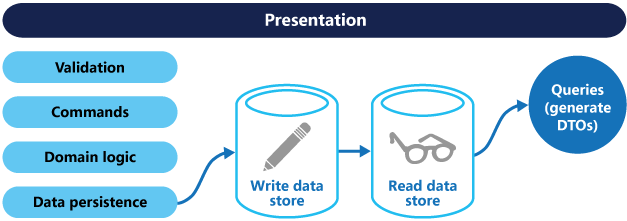
\includegraphics[width=100mm,height= 35mm, scale=1]{img/cqrs-separate-stores.png}
						\caption{CQRS Application Architecture}
					\end{figure}
			\end{itemize}
		\end{frame}
	
	\begin{frame}
		\frametitle{Data Sharing and Management}
		Command and Query Responsibility Segregation (\textbf{CQRS})
		\begin{itemize}
			\item<1->[] \small{Cloud native applications need sometimes to handle huge data.}
			\vspace{1mm}
			\item<1-> \scriptsize{In monolithic, there is no problem to handle this for simple CRUD operations}
			\item<1-> \scriptsize{Adding good managed indexes for example can solve the issue}
			\item<1-> \scriptsize{But read is not only the concern you focus on, but also writes}
			\item<1-> \scriptsize{Then, we have two concerns; \textbf{read and write}, and this is what CQRS intends to do}
			
			\item<1->[]
				\begin{figure}[h]
					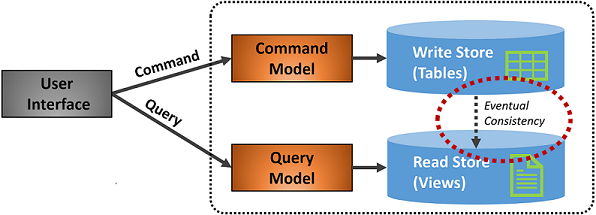
\includegraphics[width=100mm,height= 35mm, scale=1]{img/cqrs-implementation.png}
					\caption{CQRS Implementation}
				\end{figure}
		\end{itemize}
	\end{frame}


	\begin{frame}
		\frametitle{Data Sharing and Management}
		Command and Query Responsibility Segregation (\textbf{CQRS})
			\begin{itemize}
				\item<1->[] \small{Cloud native applications need sometimes to handle huge data.}
				\vspace{1mm}
				\item<1-> \scriptsize{In monolithic, there is no problem to handle this for simple CRUD operations}
				\item<1-> \scriptsize{Adding good managed indexes for example can solve the issue}
				\item<1-> \scriptsize{But read is not only the concern you focus on, but also writes}
				\item<1-> \scriptsize{Then, we have two concerns; \textbf{read and write}, and this is what CQRS intends to do}
				\item<1-> \scriptsize{\alert{You should give attention to \textbf{Eventual Consistency}}}
				\item<2->[]
					\begin{enumerate}
						\item<1-> \scriptsize{I watch the weather report and learn that it's going to rain tomorrow.}
						\item<3-> \scriptsize{I tell you that it's going to rain tomorrow.}
						\item<4-> \scriptsize{Your neighbor tells his wife that it's going to be sunny tomorrow.}
						\item<5-> \scriptsize{You tell your neighbor that it is going to rain tomorrow.	}
					\end{enumerate}
			\end{itemize}
		\vspace{100mm}
	\end{frame}

	\begin{frame}
		\frametitle{Data Sharing and Management}
		Command and Query Responsibility Segregation (\textbf{CQRS})
			\begin{itemize}
				\item<1->[] \small{Cloud native applications need sometimes to handle huge data.}
				\vspace{1mm}
				\item<1-> \scriptsize{In monolithic, there is no problem to handle this for simple CRUD operations}
				\item<1-> \scriptsize{Adding good managed indexes for example can solve the issue}
				\item<1-> \scriptsize{But read is not only the concern you focus on, but also writes}
				\item<1-> \scriptsize{Then, we have two concerns; \textbf{read and write}, and this is what CQRS intends to do}
				\item<1-> \scriptsize{However you need to make your data always in a sync mode}
				\item<1-> \scriptsize{You should give attention to \textbf{Eventual Consistency}}
				\item<1-> \scriptsize{\alert{You need also to make your query model always in a sync state}}
				\item<2-> \scriptsize{A good way to achieve this, is to use \textbf{Event Sourcing Pattern}}
					\begin{figure}[h]
						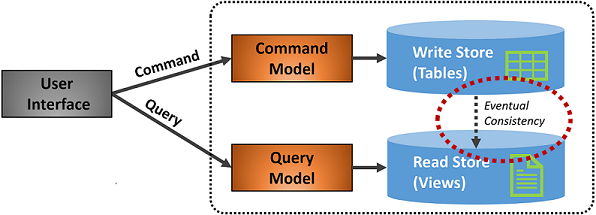
\includegraphics[width=100mm,height= 35mm, scale=1]{img/cqrs-implementation.png}
						\caption{CQRS Implementation}
					\end{figure}
			\end{itemize}
	\end{frame}

	\begin{frame}
		\frametitle{Data Sharing and Management}
			Event Sourcing Pattern
			\begin{itemize}
				\item<1->[] \scriptsize{Applying a list of events in atomic way is very hard to be applied using distributed transactions!}
				\vspace{1mm}
				\item<2-> \scriptsize{How did we get there? (\textit{History is always matter})}
				\item<3-> \scriptsize{An approach to handling operations on data that's driven by a sequence of events, each of which is recorded in an \textbf{append-only store}}
				\item<3->[]
				\begin{figure}[h]
					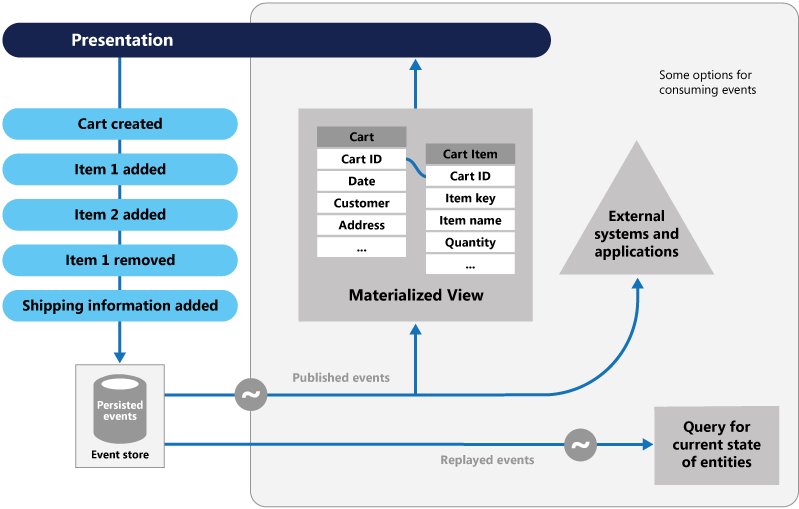
\includegraphics[width=100mm,height= 50mm, scale=1]{img/event-sourcing-overview.png}
					\caption{Event Sourcing}
				\end{figure}
		\end{itemize}
	\end{frame}
	
	\begin{frame}
	\frametitle{Data Sharing and Management}
		Event Sourcing Pattern
		\begin{itemize}
			\item<1->[] \scriptsize{By applying this pattern, you will have}
			\vspace{1mm}
			\item<2-> \scriptsize{Better performance, that is your the application code that generates the events will be decoupled from the actual code}
			\item<3-> \scriptsize{More power to scale up!}
			\item<4-> \scriptsize{Log history which is fundamental need in any project}
			\item<5-> \scriptsize{prevent concurrent updates from causing conflicts because it avoids the requirement to directly update objects in the data store}
			\item<1->[]
			\begin{figure}[h]
				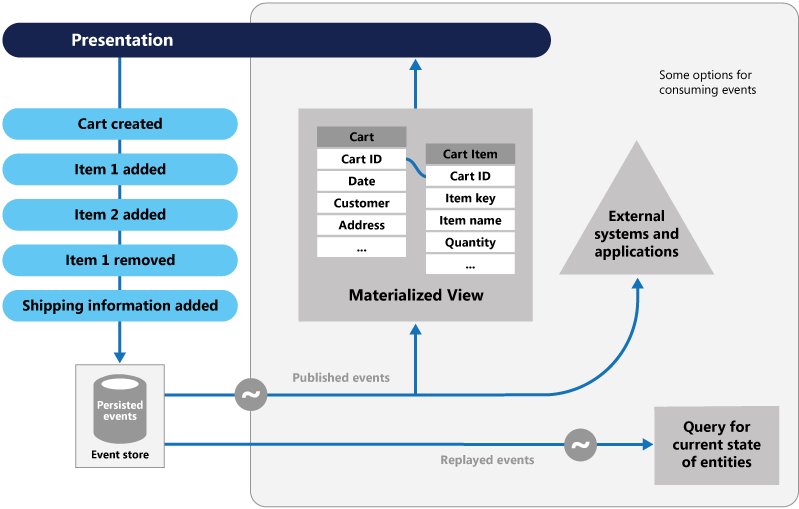
\includegraphics[width=100mm,height= 40mm, scale=1]{img/event-sourcing-overview.png}
				\caption{Event Sourcing}
			\end{figure}
		\end{itemize}
	\end{frame}

	\begin{frame}
	\frametitle{Data Sharing and Management}
		Caching Pattern
		\begin{itemize}
			\item<1->[] \scriptsize{Calling backing services is a heavy process, and to overcome this issue; you need to have some shared data store to be fully managed in run-time across all instances.}
			\vspace{1mm}
			\item<2-> \scriptsize{How can multiple instances within multiple apps share something?}
			\item<3-> \scriptsize{Why not just loading on startup? \textit{In-memory caching}}
			\item<4-> \scriptsize{Caching service is the solution. \textit{Distributed caching}}
		\end{itemize}
	\vspace{100mm}
	\end{frame}

	\begin{frame}
		\frametitle{Data Sharing and Management}
		Caching Pattern
			\begin{figure}[h]
				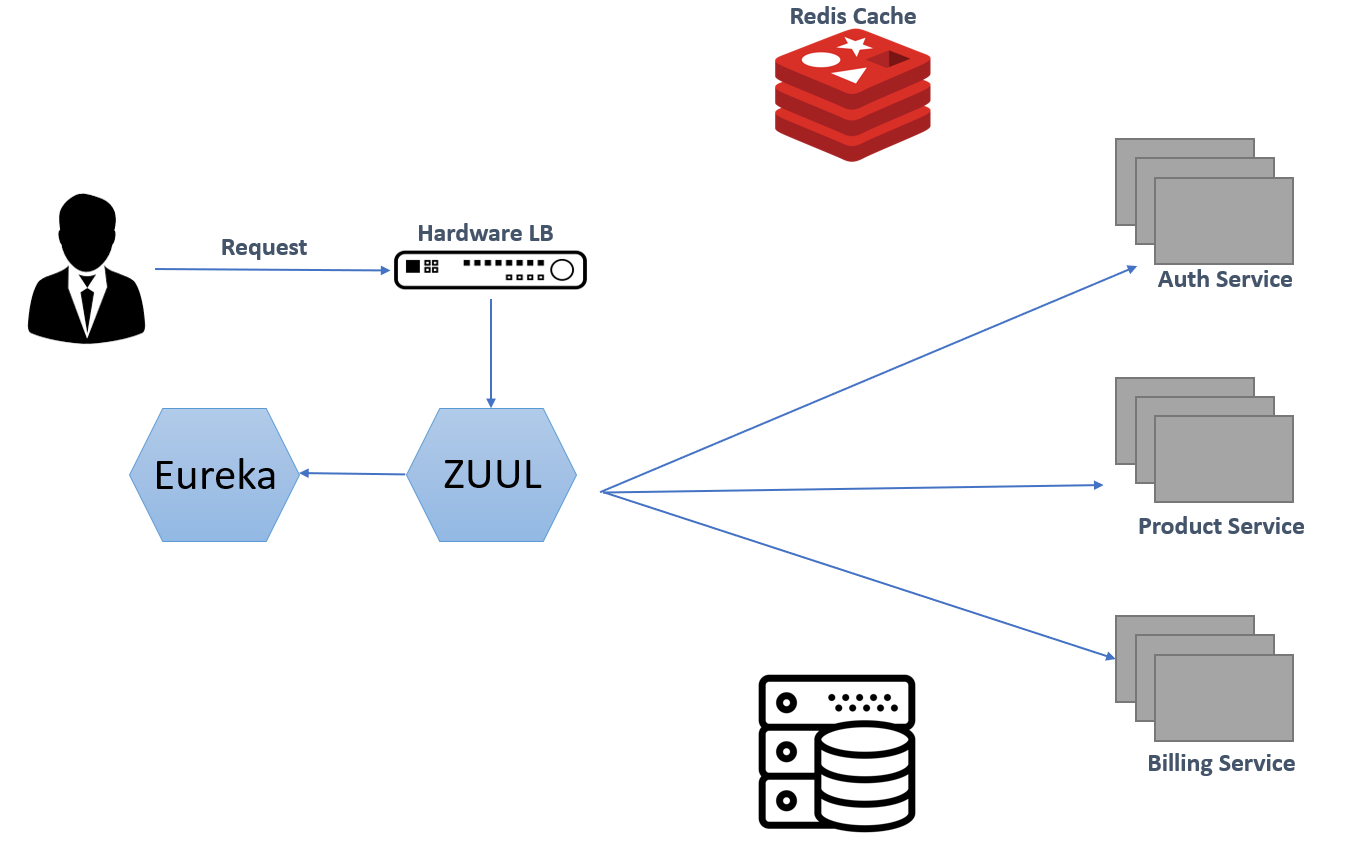
\includegraphics[width=100mm,height= 60mm, scale=1]{img/flow-1.PNG}
				\caption{Typical Scenario}
		\end{figure}
	\end{frame}

	\begin{frame}
		\frametitle{Data Sharing and Management}
		Caching Pattern
		\begin{figure}[h]
			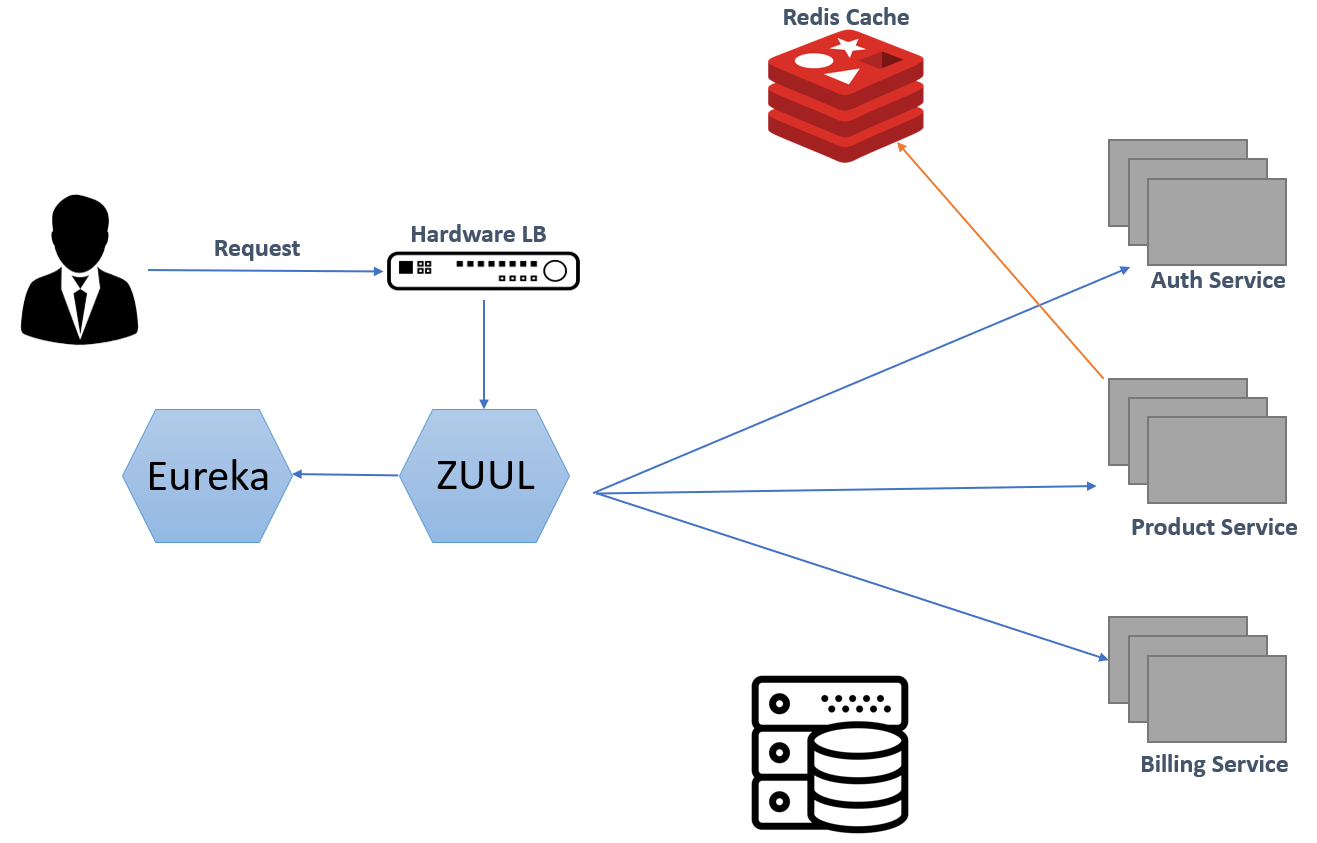
\includegraphics[width=100mm,height= 60mm, scale=1]{img/flow-2.PNG}
			\caption{Typical Scenario}
		\end{figure}
	\end{frame}

	\begin{frame}
		\frametitle{Data Sharing and Management}
		Caching Pattern
		\begin{figure}[h]
			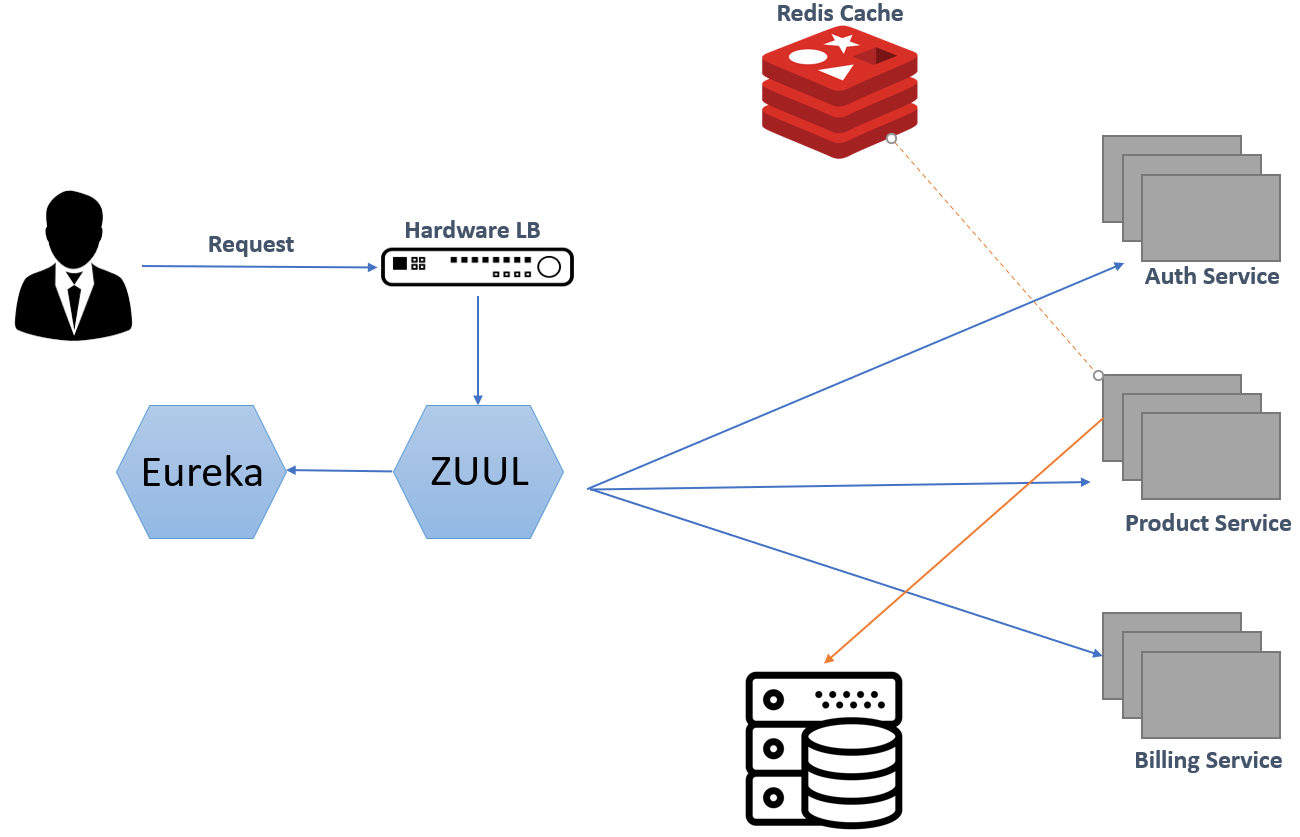
\includegraphics[width=100mm,height= 60mm, scale=1]{img/flow-3.PNG}
			\caption{Typical Scenario}
		\end{figure}
	\end{frame}

	\begin{frame}
		\frametitle{Data Sharing and Management}
		Caching Pattern
		\begin{figure}[h]
			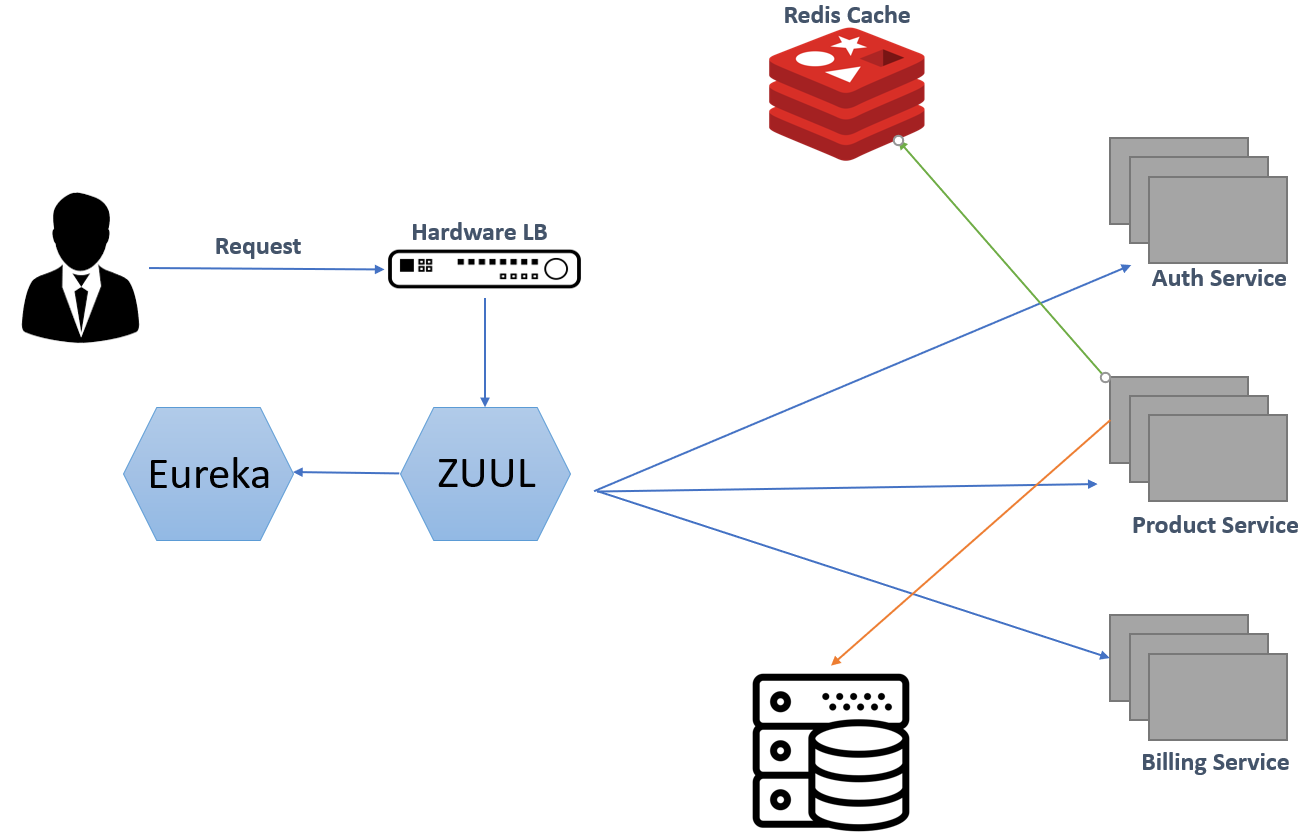
\includegraphics[width=100mm,height= 60mm, scale=1]{img/flow-4.PNG}
			\caption{Typical Scenario}
		\end{figure}
	\end{frame}


	\begin{frame}
	\frametitle{Data Sharing and Management}
	Caching Pattern
	\begin{itemize}
		\item<1->[] \scriptsize{Calling backing services is a heavy process, and to overcome this issue; you need to have some shared data store to be fully managed in run-time across all instances.}
		\vspace{1mm}
		\item<1-> \scriptsize{How can multiple instances within multiple apps share something?}
		\item<1-> \scriptsize{Why not just loading on startup? \textit{In-memory caching}}
		\item<1-> \scriptsize{Caching service is the solution. \textit{Distributed caching}}
		\item<3-> \scriptsize{\alert{You should consider also availability and data consistency}}
		\item<2->[]
		\begin{figure}[h]
			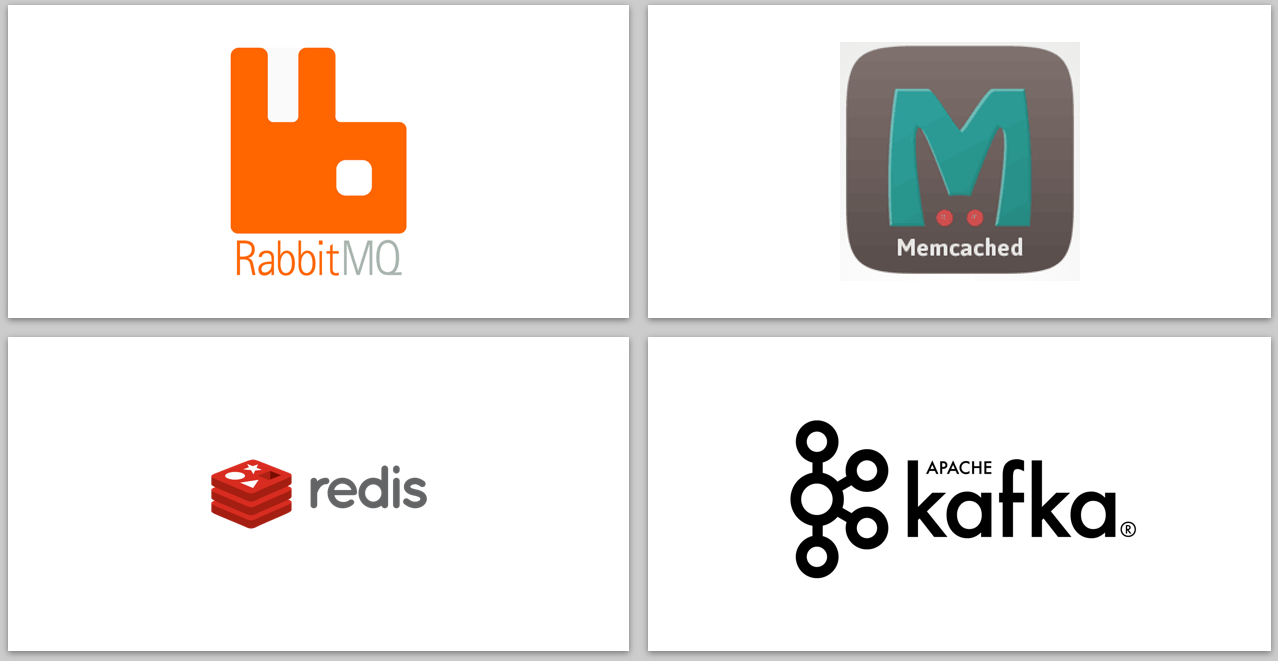
\includegraphics[width=100mm,height= 40mm, scale=1]{img/shared-ds.PNG}
			\caption{Shared DS Market Availability}
		\end{figure}
	\end{itemize}
	\end{frame}
	
	\begin{frame}
		\frametitle{The Twelve-Factor App}
		\begin{enumerate}
			\setcounter{enumi}{7}
			\item Concurrency \\
			\hspace{2mm} \scriptsize{Build your app processes like unix process model based}
			\lstinputlisting[language=Bash]{example.sh}	
			\begin{itemize}
				\item<1-> \scriptsize {Download the application, Install and Start}
				\item<1->[]
				\begin{figure}[h]
					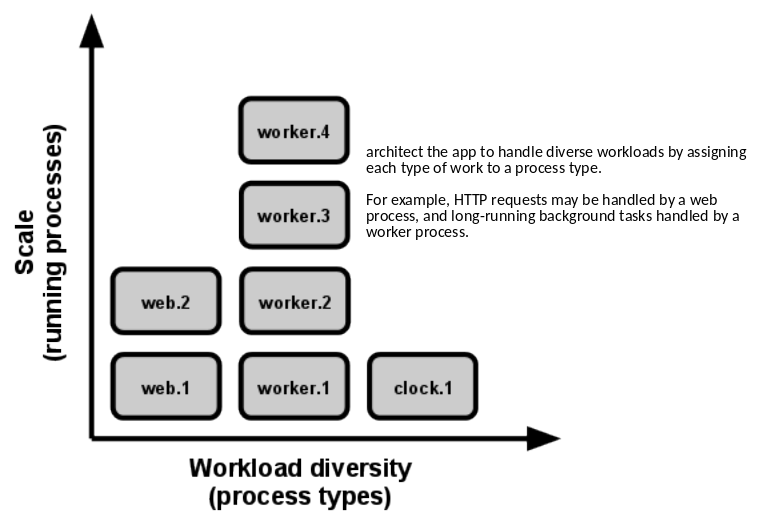
\includegraphics[width=100mm,height= 55mm, scale=1]{img/process-types.png}
				\end{figure}
			\end{itemize}
		\end{enumerate}
		\tiny{https://12factor.net/concurrency}
	\end{frame}

	\begin{frame}
		\frametitle{The Twelve-Factor App}
			\begin{enumerate}
				\setcounter{enumi}{8}
				\item Logs \\
				\begin{itemize}
					\item<1->[] \scriptsize{Logs are the app assets, and should be handled in a special way}
					\item<2-> \scriptsize {Logs are streams, and it is not the app job how to save them?}
					\item<3-> \scriptsize {A dedicated process should do this, and app work is output logs only}
					\item<4-> \scriptsize {You should give attention to what you are logging, that is you may need this data later, even on long term for analysis and reporting}
					\item<5-> \scriptsize {Today we have some good dedicated software which can aggregate files from different locations, like Logstash and Splunk}
					\item<6-> \scriptsize {Viewing the logs with reports also are different task with different good software like Kibana, Datadog, Fluentd, and others }
					\item<2->[]
					\begin{figure}[h]
						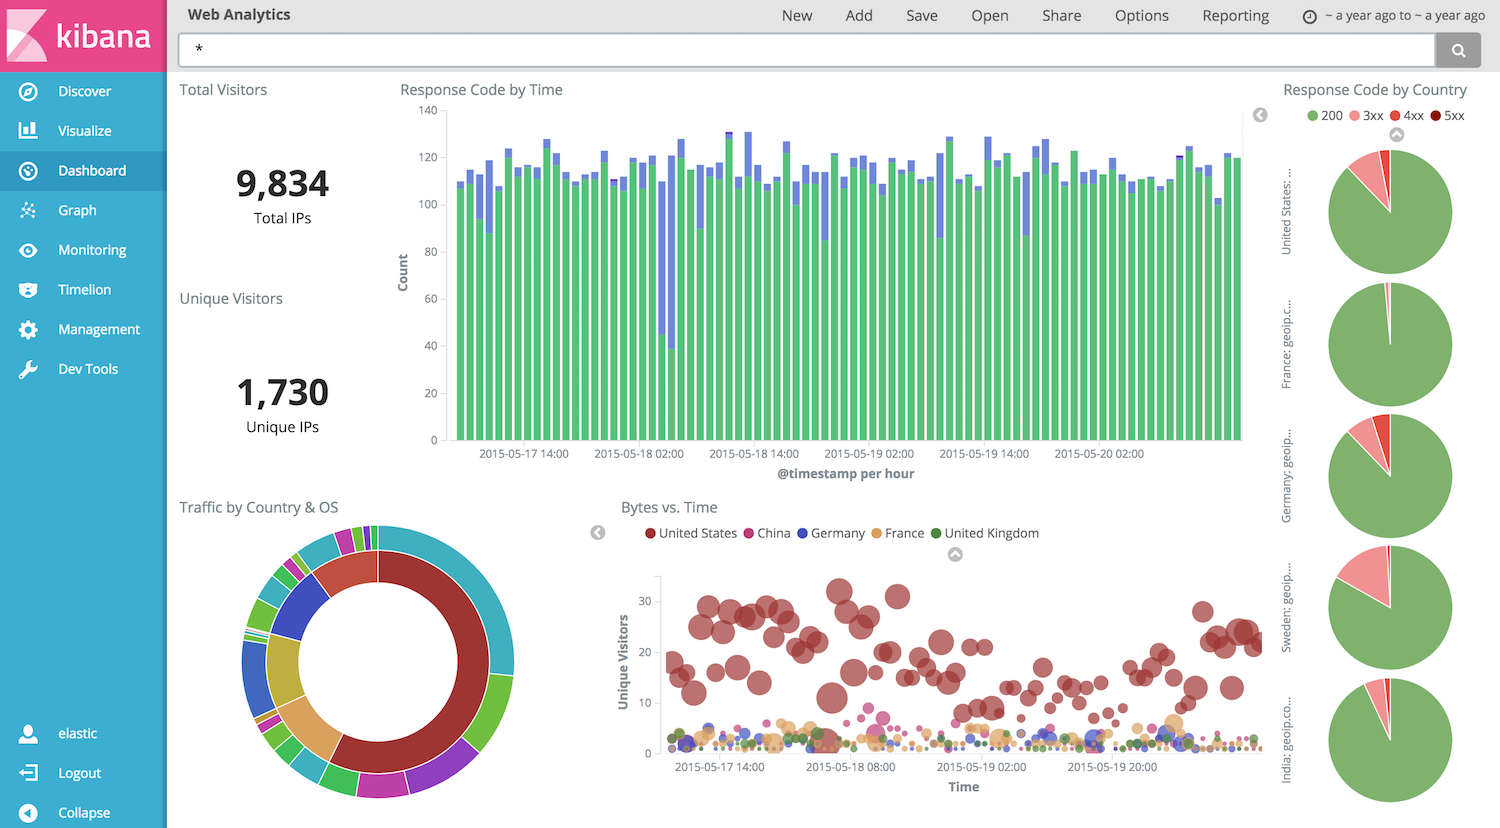
\includegraphics[width=90mm,height= 45mm, scale=1]{img/logs.png}
					\end{figure}
				\end{itemize}
			\end{enumerate}
			\vspace{100mm}
	\end{frame}
	

	\subsection {Deployment and Hosting}
		\begin{frame}
			\frametitle{Service Orchestrators}
				An orchestrator handles tasks of deploying and managing a set of services. With orchestrator you can 
				\begin{itemize}
					\item<1-> Placing services on nodes. 
					\item<2-> Monitoring the health of services and restarting unhealthy services.
					\item<3-> Load balancing network traffic across service instances. 
					\item<4-> Service discovery
					\item<5-> Scaling the number of instances of a service
					\item<6->
						\vspace{5mm}
						\begin{columns}[c]
							\column{.30\textwidth} 
							Popular Orchestrators
							\begin{itemize}
								\item Docker Swarm
								\item Kubernates
								\item Service Fabric
								\item Openshift
							\end{itemize}
							
							\column{.70\textwidth} % Right column and width
							\begin{figure}[h]
								
\includegraphics[width=70mm, height=20mm, scale=1]{img/service-orch.png}
							\end{figure}\vspace{1mm}
						\end{columns}
				\end{itemize}
			\vspace{100mm}
		\end{frame}
	
		\begin{frame}
			\frametitle{Cloud Services' Deployment}
				The old and known style is called On-Premise deployment, and it has its cons.\\
				Today we have awesome cloud tools for deployment.
				\begin{itemize}
					\item AWS
					\item Microsoft Azure
				\end{itemize}
				\vspace{100mm}
		\end{frame}

	\subsection {Monitoring}
		\begin{frame}
			\frametitle{Monitoring}
				One of the most hassle part in Microservices is \textbf{tracing}! What, How and Why this error occurred? 
				\begin{itemize}
					\item Logging 
					\item Tracing
						\begin{itemize}
							\item \scriptsize{Request may span multiple microservices, you should have some tracker over this.}
							\item \scriptsize{Trace ID is a good way to do that}
						\end{itemize}
					\item Monitor matrices 
				\end{itemize}
			\vspace{100mm}
		\end{frame}
	
		


\section{Microservices in Actions}
	\subsection {Project Structure}
	\subsection {Framework and Tools}
	
	
\begin{frame}
\frametitle{References}
\footnotesize{
\begin{thebibliography}{99} % Beamer does not support BibTeX so references must be inserted manually as below
\bibitem[Sam Newman, 2015]{p1} Sam Newman, (2015)
\newblock Building Microservices: Designing Fine-Grained Systems
\newblock \emph{O'Reilly}

\bibitem[Morgan Bruce, Paulo A. Pereira, 2018]{p1} Morgan Bruce, Paulo A. Pereira, (2085)
\newblock Microservices in Action
\newblock \emph{Manning Publications}

\bibitem[John Carnell, 2015]{p1} John Carnell, (2017)
\newblock Spring Microservices in Action
\newblock \emph{Manning Publications}

\bibitem[John Carnell, 2015]{p1} Jez Humble, David Farley (2010)
\newblock Continuous Delivery
\newblock \emph{Addison-Wesley Professional}
\end{thebibliography}
}
\end{frame}

%------------------------------------------------

\begin{frame}
\Huge{\centerline{Thanks for Watching}}
\end{frame}

%----------------------------------------------------------------------------------------

\end{document} 